%%%%%%%%%%%%%%%%%%%%%%%%%%%%%%%%%%%%%%%%
% datoteka diploma-vzorec.tex
%
% vzorčna datoteka za pisanje diplomskega dela v formatu LaTeX
% na UL Fakulteti za računalništvo in informatiko
%
% vkup spravil Gašper Fijavž, december 2010
% 
%
%
% verzija 12. februar 2014 (besedilo teme, seznam kratic, popravki Gašper Fijavž)
% verzija 10. marec 2014 (redakcijski popravki Zoran Bosnić)
% verzija 11. marec 2014 (redakcijski popravki Gašper Fijavž)
% verzija 15. april 2014 (pdf/a 1b compliance, not really - just claiming, Damjan Cvetan, Gašper Fijavž)
% verzija 23. april 2014 (privzeto cc licenca)
% verzija 16. september 2014 (odmiki strain od roba)
% verzija 28. oktober 2014 (odstranil vpisno številko)
% verija 5. februar 2015 (Literatura v kazalu, online literatura)
% verzija 25. september 2015 (angl. naslov v izjavi o avtorstvu)
% verzija 26. februar 2016 (UL izjava o avtorstvu)
% verzija 16. april 2016 (odstranjena izjava o avtorstvu)
% verzija 5. junij 2016 (Franc Solina dodal vrstice, ki jih je označil s svojim imenom)


\documentclass[a4paper, 12pt]{book}
%\documentclass[a4paper, 12pt, draft]{book}  Nalogo preverite tudi z opcijo draft, ki vam bo pokazala, katere vrstice so predolge!



\usepackage[utf8x]{inputenc}   % omogoča uporabo slovenskih črk kodiranih v formatu UTF-8
\usepackage[slovene,english]{babel}    % naloži, med drugim, slovenske delilne vzorce
\usepackage[pdftex]{graphicx}  % omogoča vlaganje slik različnih formatov
\usepackage{fancyhdr}          % poskrbi, na primer, za glave stranif
\usepackage{amssymb}           % dodatni simboli
\usepackage{amsmath}           % eqref, npr.
%\usepackage{hyperxmp}
\usepackage[hyphens]{url}  % dodal Solina
\usepackage{comment}       % dodal Solina

\usepackage[pdftex, colorlinks=true,
						citecolor=black, filecolor=black, 
						linkcolor=black, urlcolor=black,
						pagebackref=false, 
						pdfproducer={LaTeX}, pdfcreator={LaTeX}, hidelinks]{hyperref}

\usepackage{color}       % dodal Solina
\usepackage{soul}       % dodal Solina

%%%%%%%%%%%%%%%%%%%%%%%%%%%%%%%%%%%%%%%%
%	DIPLOMA INFO
%%%%%%%%%%%%%%%%%%%%%%%%%%%%%%%%%%%%%%%%
\newcommand{\ttitle}{Elektronsko naročanje v restavraciji}
\newcommand{\ttitleEn}{Diploma thesis sample}
\newcommand{\tsubject}{\ttitle}
\newcommand{\tsubjectEn}{\ttitleEn}
\newcommand{\tauthor}{Luka Horvat}
\newcommand{\tkeywords}{Slovenija, naročanje, neuspešni projekti, rešitev, spletna aplikacija}
\newcommand{\tkeywordsEn}{computer, computer, computer}


%%%%%%%%%%%%%%%%%%%%%%%%%%%%%%%%%%%%%%%%
%	HYPERREF SETUP
%%%%%%%%%%%%%%%%%%%%%%%%%%%%%%%%%%%%%%%%
\hypersetup{pdftitle={\ttitle}}
\hypersetup{pdfsubject=\ttitleEn}
\hypersetup{pdfauthor={\tauthor, matjaz.kralj@fri.uni-lj.si}}
\hypersetup{pdfkeywords=\tkeywordsEn}


 


%%%%%%%%%%%%%%%%%%%%%%%%%%%%%%%%%%%%%%%%
% postavitev strani
%%%%%%%%%%%%%%%%%%%%%%%%%%%%%%%%%%%%%%%%  

\addtolength{\marginparwidth}{-20pt} % robovi za tisk
\addtolength{\oddsidemargin}{40pt}
\addtolength{\evensidemargin}{-40pt}

\renewcommand{\baselinestretch}{1.3} % ustrezen razmik med vrsticami
\setlength{\headheight}{15pt}        % potreben prostor na vrhu
\renewcommand{\chaptermark}[1]%
{\markboth{\MakeUppercase{\thechapter.\ #1}}{}} \renewcommand{\sectionmark}[1]%
{\markright{\MakeUppercase{\thesection.\ #1}}} \renewcommand{\headrulewidth}{0.5pt} \renewcommand{\footrulewidth}{0pt}
\fancyhf{}
\fancyhead[LE,RO]{\sl \thepage} 
%\fancyhead[LO]{\sl \rightmark} \fancyhead[RE]{\sl \leftmark}
\fancyhead[RE]{\sc \tauthor}              % dodal Solina
\fancyhead[LO]{\sc Diplomska naloga}     % dodal Solina


\newcommand{\BibTeX}{{\sc Bib}\TeX}

%%%%%%%%%%%%%%%%%%%%%%%%%%%%%%%%%%%%%%%%
% naslovi
%%%%%%%%%%%%%%%%%%%%%%%%%%%%%%%%%%%%%%%%  


\newcommand{\autfont}{\Large}
\newcommand{\titfont}{\LARGE\bf}
\newcommand{\clearemptydoublepage}{\newpage{\pagestyle{empty}\cleardoublepage}}
\setcounter{tocdepth}{2}	      % globina kazala

%%%%%%%%%%%%%%%%%%%%%%%%%%%%%%%%%%%%%%%%
% konstrukti
%%%%%%%%%%%%%%%%%%%%%%%%%%%%%%%%%%%%%%%%  
\newtheorem{izrek}{Izrek}[chapter]
\newtheorem{trditev}{Trditev}[izrek]
\newenvironment{dokaz}{\emph{Dokaz.}\ }{\hspace{\fill}{$\Box$}}

%%%%%%%%%%%%%%%%%%%%%%%%%%%%%%%%%%%%%%%%%%%%%%%%%%%%%%%%%%%%%%%%%%%%%%%%%%%%%%%
%% PDF-A
%%%%%%%%%%%%%%%%%%%%%%%%%%%%%%%%%%%%%%%%%%%%%%%%%%%%%%%%%%%%%%%%%%%%%%%%%%%%%%%


%%%%%%%%%%%%%%%%%%%%%%%%%%%%%%%%%%%%%%%% 
% define medatata
%%%%%%%%%%%%%%%%%%%%%%%%%%%%%%%%%%%%%%%% 
\def\Title{\ttitle}
\def\Author{\tauthor, lh8069@fri.uni-lj.si}
\def\Subject{\ttitleEn}
\def\Keywords{\tkeywordsEn}

%%%%%%%%%%%%%%%%%%%%%%%%%%%%%%%%%%%%%%%% 
% \convertDate converts D:20080419103507+02'00' to 2008-04-19T10:35:07+02:00
%%%%%%%%%%%%%%%%%%%%%%%%%%%%%%%%%%%%%%%% 
\def\convertDate{%
    \getYear
}

{\catcode`\D=12
 \gdef\getYear D:#1#2#3#4{\edef\xYear{#1#2#3#4}\getMonth}
}
\def\getMonth#1#2{\edef\xMonth{#1#2}\getDay}
\def\getDay#1#2{\edef\xDay{#1#2}\getHour}
\def\getHour#1#2{\edef\xHour{#1#2}\getMin}
\def\getMin#1#2{\edef\xMin{#1#2}\getSec}
\def\getSec#1#2{\edef\xSec{#1#2}\getTZh}
\def\getTZh +#1#2{\edef\xTZh{#1#2}\getTZm}
\def\getTZm '#1#2'{%
    \edef\xTZm{#1#2}%
    \edef\convDate{\xYear-\xMonth-\xDay T\xHour:\xMin:\xSec+\xTZh:\xTZm}%
}

\expandafter\convertDate\pdfcreationdate 

%%%%%%%%%%%%%%%%%%%%%%%%%%%%%%%%%%%%%%%%
% get pdftex version string
%%%%%%%%%%%%%%%%%%%%%%%%%%%%%%%%%%%%%%%% 
\newcount\countA
\countA=\pdftexversion
\advance \countA by -100
\def\pdftexVersionStr{pdfTeX-1.\the\countA.\pdftexrevision}


%%%%%%%%%%%%%%%%%%%%%%%%%%%%%%%%%%%%%%%%
% XMP data
%%%%%%%%%%%%%%%%%%%%%%%%%%%%%%%%%%%%%%%%  
\usepackage{xmpincl}
\includexmp{pdfa-1b}

%%%%%%%%%%%%%%%%%%%%%%%%%%%%%%%%%%%%%%%%
% pdfInfo
%%%%%%%%%%%%%%%%%%%%%%%%%%%%%%%%%%%%%%%%  
\pdfinfo{%
    /Title    (\ttitle)
    /Author   (\tauthor, damjan@cvetan.si)
    /Subject  (\ttitleEn)
    /Keywords (\tkeywordsEn)
    /ModDate  (\pdfcreationdate)
    /Trapped  /False
}


%%%%%%%%%%%%%%%%%%%%%%%%%%%%%%%%%%%%%%%%%%%%%%%%%%%%%%%%%%%%%%%%%%%%%%%%%%%%%%%
%%%%%%%%%%%%%%%%%%%%%%%%%%%%%%%%%%%%%%%%%%%%%%%%%%%%%%%%%%%%%%%%%%%%%%%%%%%%%%%

\begin{document}
\selectlanguage{slovene}
\frontmatter
\setcounter{page}{1} %
\renewcommand{\thepage}{}       % preprecimo težave s številkami strani v kazalu
\newcommand{\sn}[1]{"`#1"'}                    % dodal Solina (slovenski narekovaji)

%%%%%%%%%%%%%%%%%%%%%%%%%%%%%%%%%%%%%%%%
%naslovnica
 \thispagestyle{empty}%
   \begin{center}
    {\large\sc Univerza v Ljubljani\\%
      Fakulteta za računalništvo in informatiko}%
    \vskip 10em%
    {\autfont \tauthor\par}%
    {\titfont \ttitle \par}%
    {\vskip 3em \textsc{DIPLOMSKO DELO\\[5mm]         % dodal Solina za ostale študijske programe
%    VISOKOŠOLSKI STROKOVNI ŠTUDIJSKI PROGRAM\\ PRVE STOPNJE\\ RAČUNALNIŠTVO IN INFORMATIKA}\par}%
    VISOKOŠOLSKI ŠTUDIJSKI PROGRAM \\ PRVE STOPNJE\\ RAČUNALNIŠTVO IN INFORMATIKA}\par}%
%    INTERDISCIPLINARNI UNIVERZITETNI\\ ŠTUDIJSKI PROGRAM PRVE STOPNJE\\ RAČUNALNIŠTVO IN MATEMATIKA}\par}%
%    INTERDISCIPLINARNI UNIVERZITETNI\\ ŠTUDIJSKI PROGRAM PRVE STOPNJE\\ UPRAVNA INFORMATIKA}\par}%
%    INTERDISCIPLINARNI UNIVERZITETNI\\ ŠTUDIJSKI PROGRAM PRVE STOPNJE\\ MULTIMEDIJA}\par}%
    \vfill\null%
    {\large \textsc{Mentorica}: doc. dr. Mira Trebar\par}%
   {\large \textsc{Somentor}: as. dr. David Jelenc \par}%
    {\vskip 2em \large Ljubljana, 2021 \par}%
\end{center}
% prazna stran
%\clearemptydoublepage      % dodal Solina (izjava o licencah itd. se izpiše na hrbtni strani naslovnice)

%%%%%%%%%%%%%%%%%%%%%%%%%%%%%%%%%%%%%%%%
%copyright stran
\thispagestyle{empty}
\vspace*{8cm}

\noindent
{\sc Copyright}. 
Rezultati diplomske naloge so intelektualna lastnina avtorja in Fakultete za računalništvo in informatiko Univerze v Ljubljani.
Za objavo in koriščenje rezultatov diplomske naloge je potrebno pisno privoljenje avtorja, Fakultete za računalništvo in informatiko ter mentorja.

\begin{center}
\mbox{}\vfill
\emph{Besedilo je oblikovano z urejevalnikom besedil \LaTeX.}
\end{center}
% prazna stran
\clearemptydoublepage

%%%%%%%%%%%%%%%%%%%%%%%%%%%%%%%%%%%%%%%%
% stran 3 med uvodnimi listi
\thispagestyle{empty}
\vspace*{4cm}

\noindent
Fakulteta za računalništvo in informatiko izdaja naslednjo nalogo:
\medskip
\begin{tabbing}
\hspace{32mm}\= \hspace{6cm} \= \kill




Tematika naloge: Elektronsko naročanje v restavracij
\end{tabbing}
Besedilo teme diplomskega dela študent prepiše iz študijskega informacijskega sistema, kamor ga je vnesel mentor. V nekaj stavkih bo opisal, kaj pričakuje od kandidatovega diplomskega dela. Kaj so cilji, kakšne metode uporabiti, morda bo zapisal tudi ključno literaturo.
\vspace{15mm}






\vspace{2cm}

% prazna stran
\clearemptydoublepage

% zahvala
\thispagestyle{empty}\mbox{}\vfill\null\it%
\noindent
Na tem mestu zapišite, komu se zahvaljujete za izdelavo diplomske naloge. Pazite, da ne boste koga pozabili. Utegnil vam bo zameriti. Temu se da izogniti tako, da celotno zahvalo izpustite.
\rm\normalfont

% prazna stran
\clearemptydoublepage

%%%%%%%%%%%%%%%%%%%%%%%%%%%%%%%%%%%%%%%%
% posvetilo, če sama zahvala ne zadošča :-)
%\thispagestyle{empty}\mbox{}{\vskip0.20\textheight}\mbox{}\hfill\begin{minipage}{0.55\textwidth}%
%Svoji dragi Alenčici.
%\normalfont\end{minipage}

% prazna stran
\clearemptydoublepage


%%%%%%%%%%%%%%%%%%%%%%%%%%%%%%%%%%%%%%%%
% kazalo
\pagestyle{empty}
\def\thepage{}% preprecimo tezave s stevilkami strani v kazalu
\tableofcontents{}

% prazna stran
\clearemptydoublepage

%%%%%%%%%%%%%%%%%%%%%%%%%%%%%%%%%%%%%%%%
% seznam kratic

\chapter*{Seznam uporabljenih kratic}  % spremenil Solina, da predolge vrstice ne gredo preko desnega roba

\begin{comment}
\begin{tabular}{l|l|l}
  {\bf kratica} & {\bf angleško} & {\bf slovensko} \\ \hline
  % after \\: \hline or \cline{col1-col2} \cline{col3-col4} ...
  {\bf SPA} & single page application & aplikacija na eni strani \\
  {\bf SQL} & structured query language & strukturirani povpraševalni jezik za delo s podatkovnimi bazami  \\
  {\bf SVM} & support vector machine & metoda podpornih vektorjev \\
  {\bf SVM}   & support vector machine              & metoda podpornih vektorjev \\
  \dots & \dots & \dots \\
\end{tabular}
\end{comment}

\noindent\begin{tabular}{p{0.1\textwidth}|p{.4\textwidth}|p{.4\textwidth}}    % po potrebi razširi prvo kolono tabele na račun drugih dveh!
  {\bf kratica} & {\bf angleško}                             & {\bf slovensko} \\ \hline
  {\bf SPA}      & single page application               &  aplikacija na eni strani \\
  {\bf SQL} & structured query language & strukturirani povpraševalni jezik za delo s podatkovnimi bazami  \\
  {\bf CLI}   & command-line interface              & znakovni uporabniški vmesnik \\
  {\bf REST}   & representational state transfer              & aktualni prenos stanja \\
  {\bf URI}   &  uniform resource identifier              & enotni identifikator vira \\
  {\bf SPA}   &  single-page application              & aplikacija na eni strani \\
  {\bf HTTP}   &  hypertext transfer protocol               & protokol za prenos hiperteksta \\
  {\bf SUPB}   &  database management system              & sistem za upravljanje s podatkovno bazo \\
  {\bf API}   &  application programming interface              & programski vmesnik\\
  {\bf QR}   &  qucik  response              & hiter odziv\\
%  \dots & \dots & \dots \\
\end{tabular}


% prazna stran
\clearemptydoublepage

%%%%%%%%%%%%%%%%%%%%%%%%%%%%%%%%%%%%%%%%
% povzetek
\addcontentsline{toc}{chapter}{Povzetek}
\chapter*{Povzetek}

\noindent\textbf{Naslov:} \ttitle
\bigskip

\noindent\textbf{Avtor:} \tauthor
\bigskip


%\noindent\textbf{Povzetek:} 
\noindent 
Diplomsko delo zajema analizo, načrtovanje in razvoj spletne aplikacije, ki je namenjena elektronskemu naročanju hrane in pijače v restavracijah. Namen aplikacije je olajšati delo natakarjem in nuditi bolj kakovostno postrežbo gostom. Ključne funkcionalnosti so oddajanje naročil s strani gosta ter nadzor in upravljanje naročil s strani natakarja in kuharja. Omogočeno je naročanje preko aplikacije ali z neposrednim stikom z natakarjem. Aplikacija je zasnovana po visokonivojski arhitekturi, ki jo sestavljajo aplikacija, strežnik in podatkovna baza. Za razvoj aplikacije se je uporabil programski jezik JavaScript in ogrodje Vue, za strežnik Python in MySQL za podatkovno bazo. Razvita rešitev je pripravljena za implementacijo v restavracijah.
\bigskip

\noindent\textbf{Ključne besede:} \tkeywords.
% prazna stran
\clearemptydoublepage

%%%%%%%%%%%%%%%%%%%%%%%%%%%%%%%%%%%%%%%%
% abstract
\selectlanguage{english}
\addcontentsline{toc}{chapter}{Abstract}
\chapter*{Abstract}

\noindent\textbf{Title:} \ttitleEn
\bigskip

\noindent\textbf{Author:} \tauthor
\bigskip

%\noindent\textbf{Abstract:} 
\noindent This sample document presents an approach to typesetting your BSc thesis using \LaTeX. 
A proper abstract should contain around 100 words which makes this one way too short.
\bigskip

\noindent\textbf{Keywords:} \tkeywordsEn.
\selectlanguage{slovene}
% prazna stran
\clearemptydoublepage

%%%%%%%%%%%%%%%%%%%%%%%%%%%%%%%%%%%%%%%%
\mainmatter
\setcounter{page}{1}
\pagestyle{fancy}
 
\chapter{Uvod}
Slovenija velja za državo z veliko restavracij, vendar le malo iz med njih uporablja napredne sisteme naročanja kot npr. ena izmed večjih verig s hitro prehrano, McDonalds. V Sloveniji so obstajali projekti s podobnimi idejami, vendar z napačnimi cilji zaradi katerih so bili neuspešni. Eden izmed glavnih razlogov, da jim ni uspelo, je bilo sabotiranje s strani natakarjev, saj so misli da bo tehnologija zamenjala njegove službe. Z zavedanjem teh problematik smo se odločili narediti diplomsko nalogo na to tematiko. 

Zamislili smo si sistem za oddajanje naročil v restavracijah, ki ne bi bil namenjen zamenjavi ljudi v strežbi, temveč kot pregledovalnik ponudbe z možnostjo naročanja hrane in pijače. Aplikacija za stranke bi bila na tablicah, ki bi bile locirane na vsaki mizi restavracije. Stranka bi bila tista, ki bi se odločala ali želi pri naročanju uporabiti stik z osebo v strežbi ali bi naročila z uporabo aplikacije na tablici. Natakar bi tako imel več časa, katerega bi lahko posvetil pripravi pijače, kvaliteti postrežbe in ostalih dolžnosti. Tudi stranke, katere sedaj veljajo za bolj zahtevne in neučakane na vseh področijh, bi bile hitreje in bolj kvalitetno postrežene. Tako bi imeli poleg restavracij s hitro prehrano tudi restavracije s hitro postrežbo. 


Aplikacija podpira tri uporabniške vloge, in sicer gost, natakar in kuhar. 

\chapter{Načrtovanje in razvoj aplikacije}

Razvoj aplikacije je potekal v treh delih in sicer analiza zahtev oziroma izdelava diagrama primerov uporabe, načrtovanje arhitekture in izbira tehnologij ter implementacija.
Rešitev sestavljajo dve aplikaciji. Ena aplikacija je namenjena gostom, druga pa natakarjem in kuharjem. Restavracija ima lahko več miz, vendar za eno mizo je lahko hkrati odprto eno naročilo. To pomeni, da morajo vsi gosti za mizo naročati skupaj. 

Gost lahko odda, spremeni ali zaključi naročilo. Funkcionalnosti gosta so: dodajanje in brisanje artiklov iz naročila, oddajanje, urejanje in pregledovanje naročila, spremljanje statusa naročila in zahtevanje računa. V restavraciji je lahko več natakarjev, ki svoje delo opravljajo istočasno. Funkcionalnosti natakarja so: dodajanje in brisanje artiklov iz naročila, urejanje in pregledovanje naročila, spremljanje statusa naročila, spremljanje statistke naročil in možnost tiskanja računa za določeno naročilo. Kuhar lahko sprejeme ali zavrne naročilo. Restavracija ima lahko več kuharjev, vendar vsi uporabljajo aplikacijo preko iste prijave. Omejitev je v podatkovnem modelu. Funkcionalnosti kuharja so: pregledovanje in potrjevanje naročila, obveščanje natakarja o zaključku priprave jedi ter spremljanje statistke naročil. 
\begin{figure}[!htb]
\begin{center}
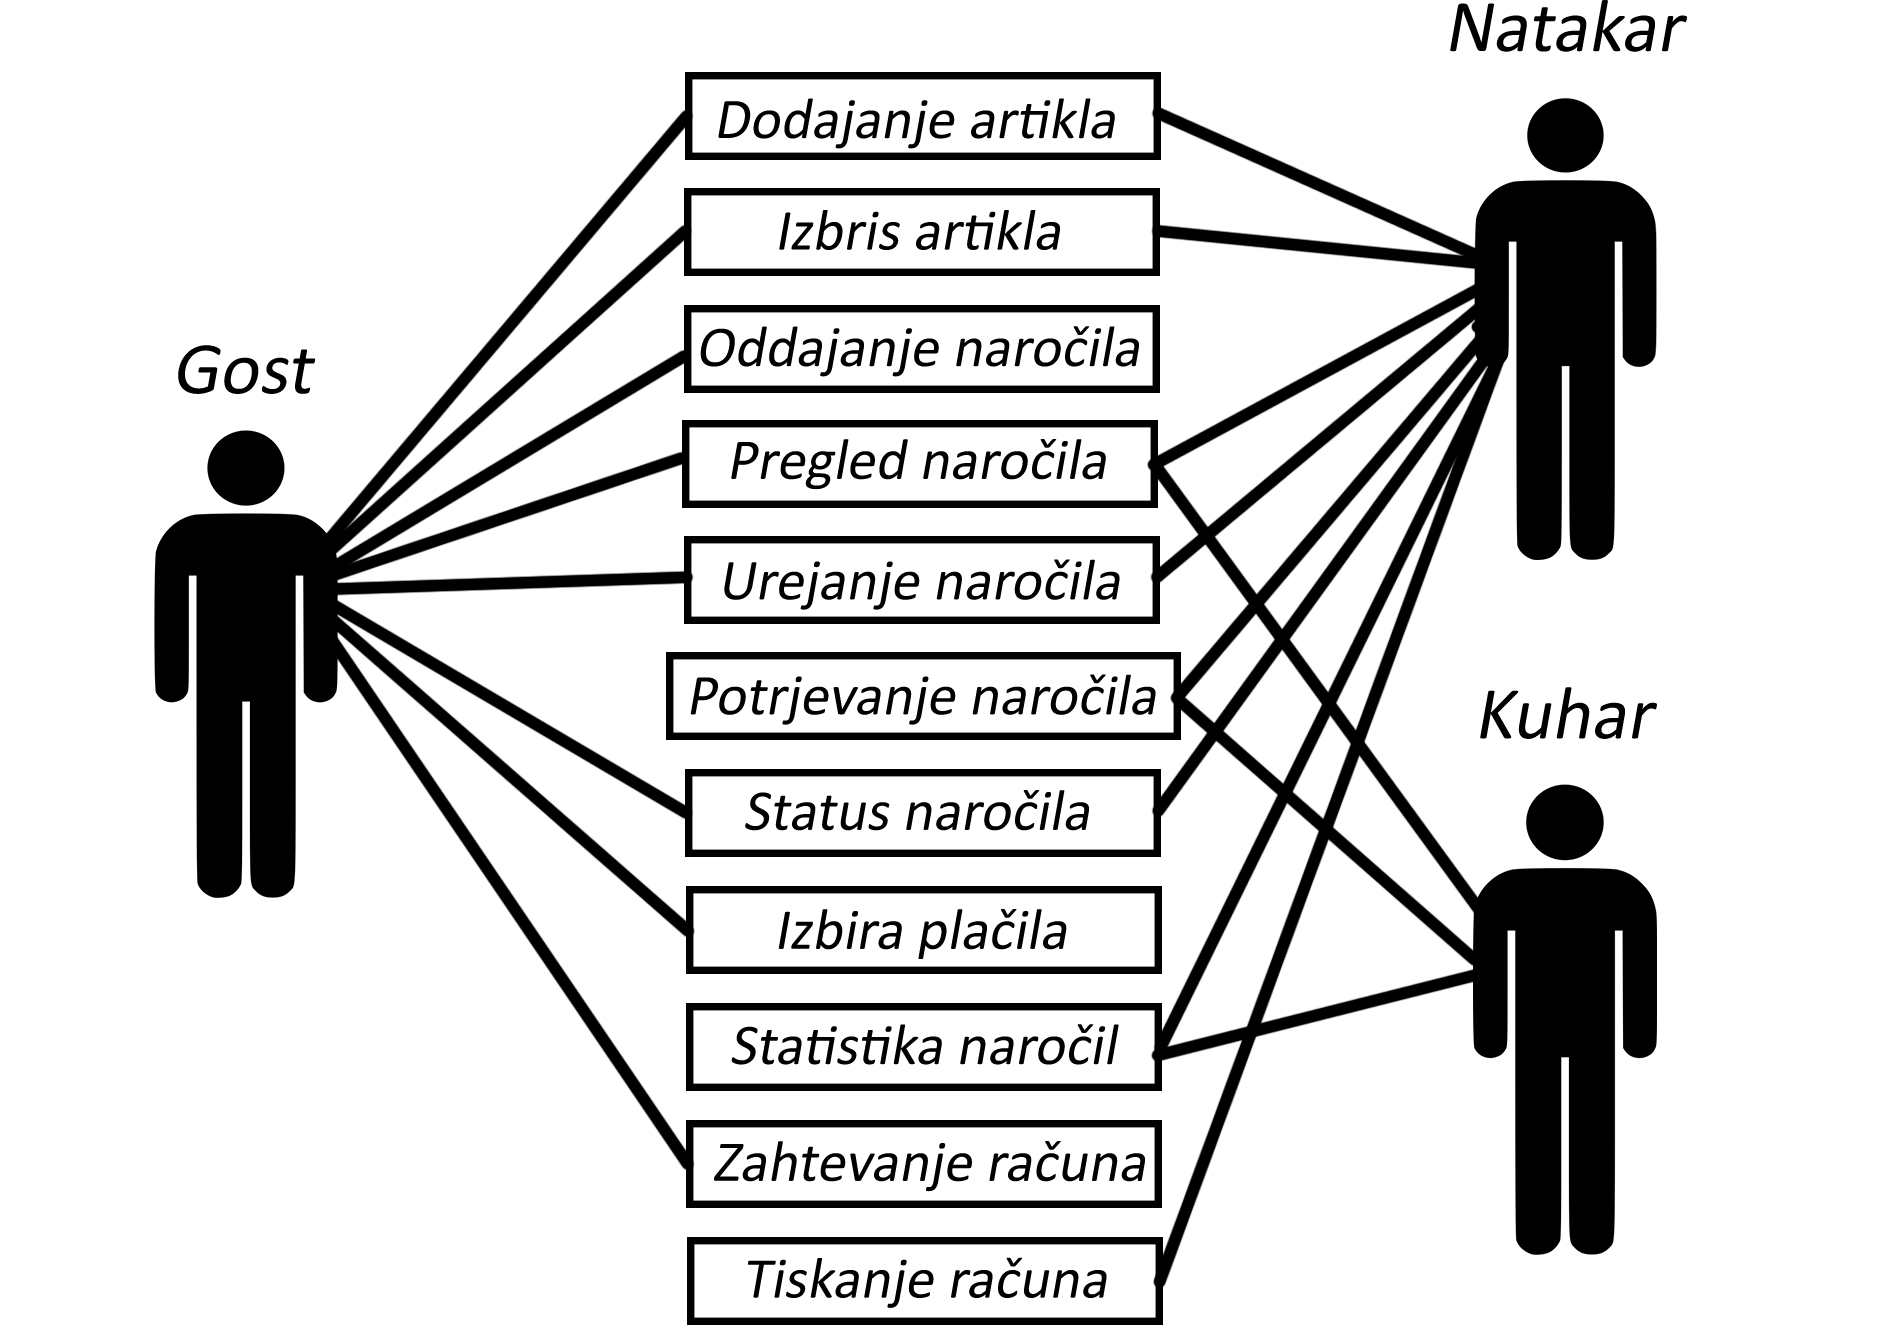
\includegraphics[width=11.5cm]{Skica2.png}
\caption{Diagram primerov uporabe spretnega naročanja}
\label{FunkVloge}
\end{center}
\end{figure}


Uporabili smo arhitekturo novodobnih aplikacij katero sestavljajo podatkovna baza, strežnik in aplikacija oziroma odjemalec. Gre za koncept, ki ga je moč prilagajati predvsem z uporabniškega vidika. Slika~\ref{StrukApk} prikazuje arhitekturno rešitev aplikacije \cite{TRINIVO}.
Podatkovna baza je namenjena shranjevanju vseh podatkov za posamezno restavracijo. Strežnik implementira vmesnik RESTful, ki odjemalcu oziroma aplikaciji posreduje podatke iz podatkovne baze. 

\begin{figure}[!htb]
\centering
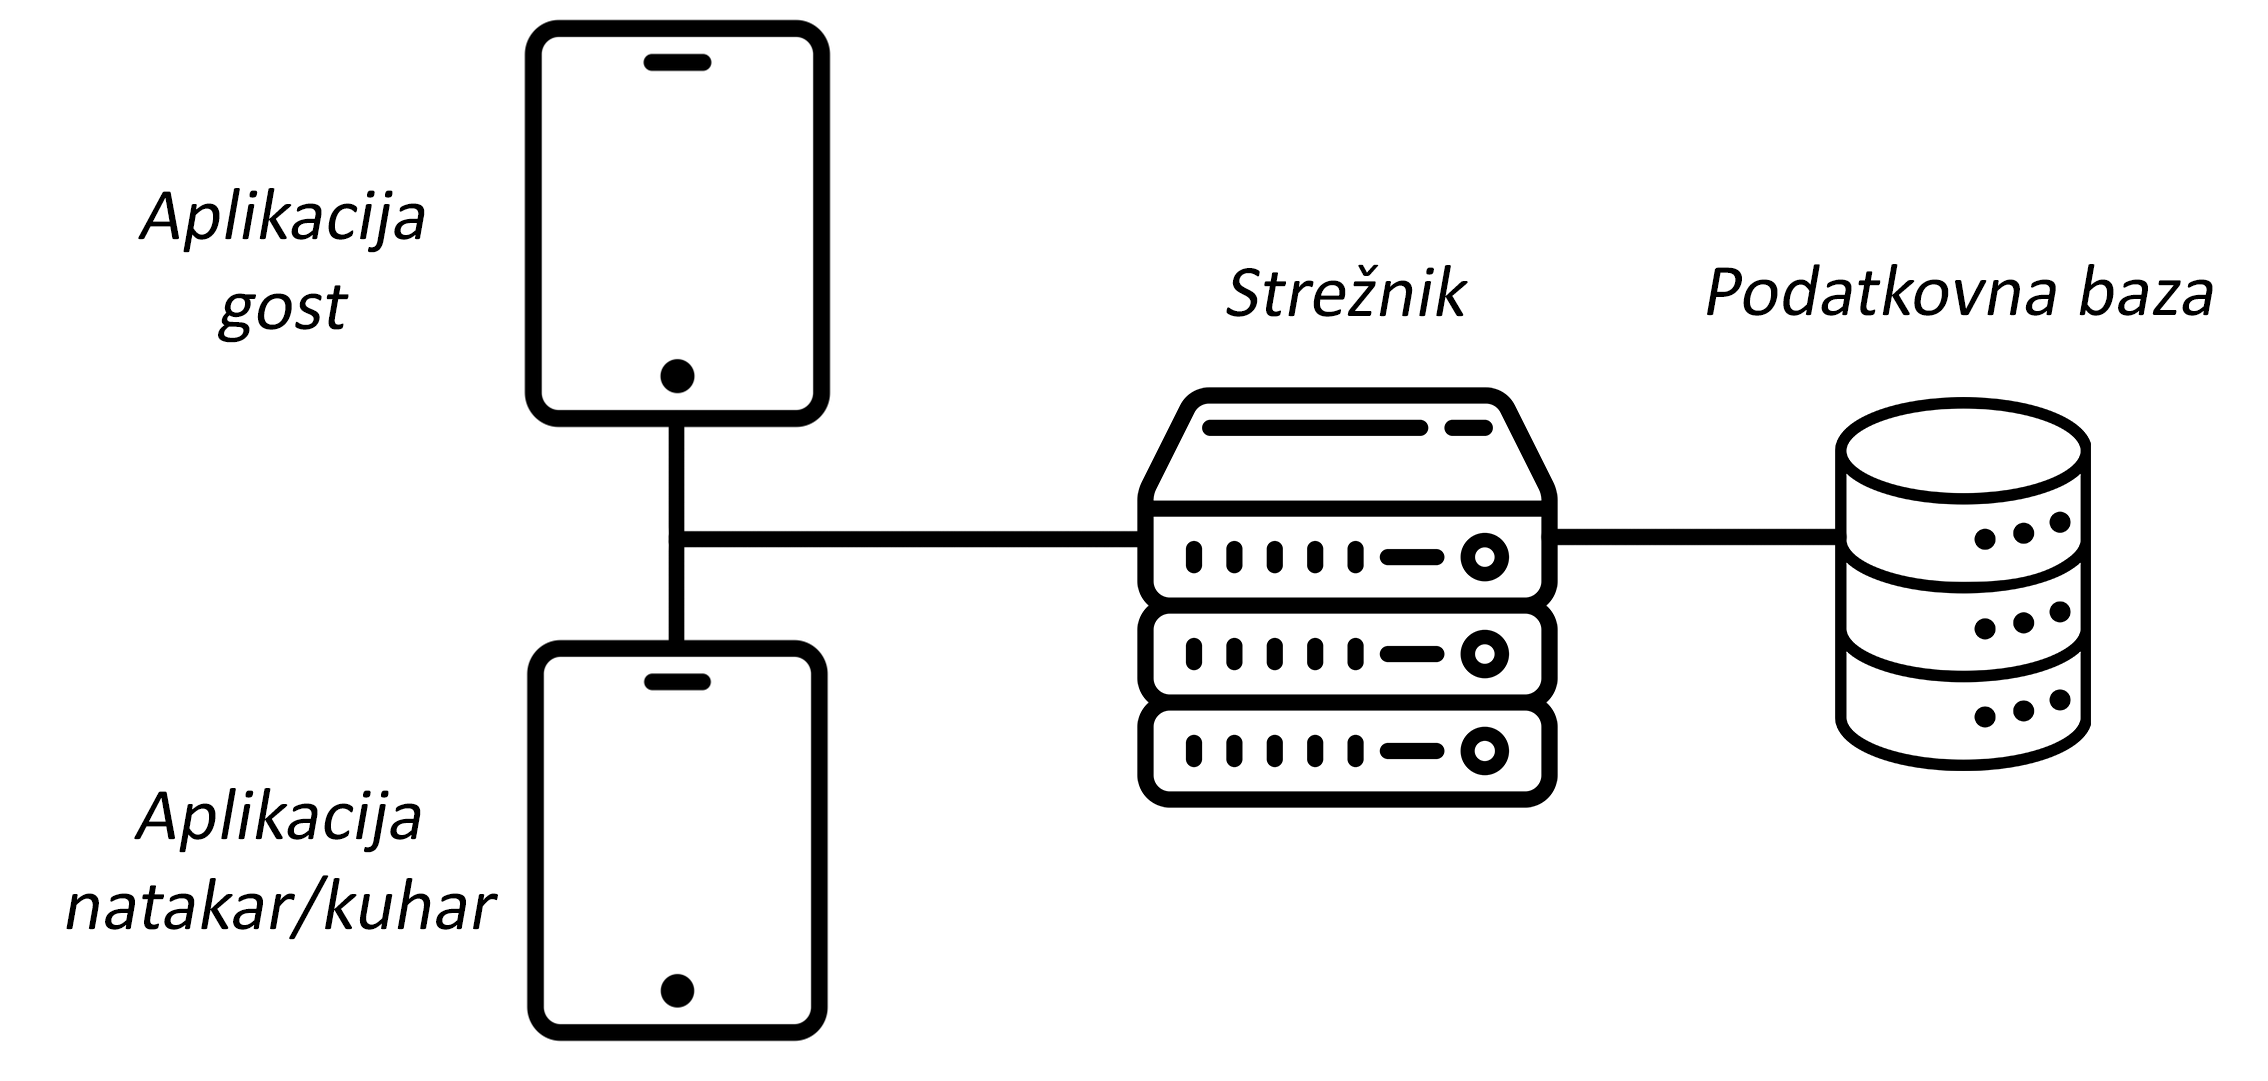
\includegraphics[width=10.5cm]{Skica1-new.png}
\caption{Visokonivojska arhitektura}
\label{StrukApk}
\end{figure}


\section{Podatkovna baza}
Na podlagi izdelanega diagrama zahtev oziroma funkcij smo najprej izdelali logičen podatkovni model (slika~\ref{Database_physical}). Podatkovna baza je sestavljena iz šestih tabel, ki so: \textit{ProductType, Product, ProductOrder, Order, User, Table}. 

\begin{figure}[!htb]
\begin{center}
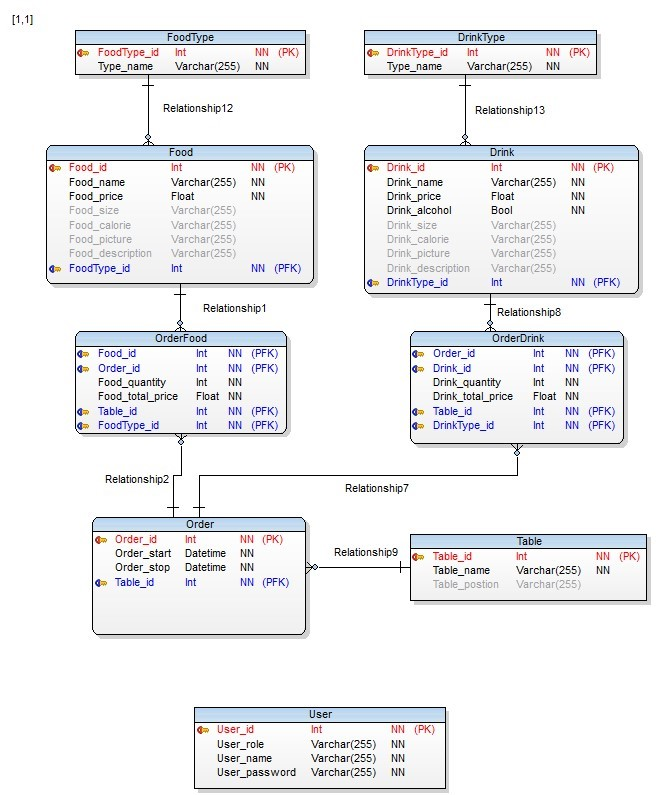
\includegraphics[width=12.5cm]{Database_physical}
\caption{Logični podatkovni model}
\label{Database_physical}
\end{center}
\end{figure}

Tabela \textit{ProductType} je namenjana zapisom za vrste jedi (predjed, glavna jed, sladica) in pijač (sokovi, piva, vina, ...). Sestavljena je iz atributov: \textit{ID}, \textit{Name} in \textit{Type}. Atribut \textit{Type} je namenjen razlikovanju hrane in pijače v naročilu.

Tabela \textit{Product} je namenjena opisu hrane in pijače ter je sestavljena iz atributov: \textit{ID}, \textit{Name}, \textit{Price}, \textit{Size}, \textit{Calorie}, \textit{Picture} in \textit{Description}. V vrednost atributa \textit{Picture} se zapiše ime slike, ki se prikaže v aplikaciji. Vse slike so shranjene v datotečnem sistemu spletnega strežnika.

Tabela \textit{ProductOrder} je namenjena količini in končni ceni hrane in pijače v naročilu. Sestavljena je iz atributov: \textit{TotalPrice} in \textit{Quantity}. Zapis ne obstaja, če nima definiranega naročila. Tabela je nastala zaradi razmerja M:N t.i. mnogo-proti-mnogo med tabelo \textit{Product} in \textit{Order}.

Tabela \textit{Order} je namenjena zapisovanju naročil in njegovih podrobnosti. Sestavljena je iz atributov: \textit{ID}, \textit{Start}, \textit{End}, \textit{OrderStatus}, \textit{CookStatus} in \textit{Payment}. Vsebuje tudi tuji ključ od tabele \textit{Table}, ki določa, na katero mizo je vezano naročilo. Atributa \textit{OrderStatus} in \textit{CookStatus} sta ENUM podatkovnega tip (preddefinirane vrednosti) in sporočata status naročila med vlogami.

Tabela \textit{Table} je namenjena označevanju miz v restavracijah. Sestavljajo jo atributi: \textit{ID}, \textit{Name} in \textit{Position}, v katerega se lahko bolj podrobno opiše lokacija mize.

Tabela \textit{User} je namenjena predvsem aplikativnemu delu za natakarje in kuharje. Sestavljna je iz atributov: \textit{ID}, \textit{Role}, \textit{Name} in \textit{Password}. 

Strukturo podatkovne baze smo definirali s pomočjo programa Toad DataModeler. To je orodje za izdelavo visokokakovostnih podatkovnih modelov \cite{Toad_Data_Modeler}. Omogoča izdelavo logičnih in fizičnih podatkovnih modelov, kar pripomore k lažjem razumevanju in razvijanju podatkovne baze. Njegova najboljša funkcionalnost je, da lahko generiramo SQL kodo v različne podatkovne sisteme kot npr. MySQL, Ingres, Microsoft Azurem, Microsoft Access in Mircrosoft SQL Server.

Podatkovni model smo implementirali na fizičnem nivoju v sistemu za upravljanje s podatkovno bazo (DBMS), ang. database management system (SUPB), MySQL. To je eden od odprtokodnih sistemov za upravljanje s podatkovni bazami, ki za delo s podatki uporablja jezik SQL (ang. structured query language) \cite{MySQL}. Napisan je v programskem jeziku C in C++ in deluje v vseh modernih operacijskih sistemih (Windows, Linux, IOS in drugih).


\section{Strežnik}
Strežnik predstavlja vmesnik med podatkovno bazo in odjemalcem. Najbolj pomembno je, da je sistem zanesljiv, saj odjemalec brez njega ne more delovati. Izbrali smo arhitekturo REST zaradi načel, ki so opisana spodaj \cite{RESTAPI}. Sama arhitektura omogoča, da odjemalec s pomočjo zahtev pridobiva podatke od strežnika, kateri jih s pomočjo povezav URI (ang. uniform resource identifier) oglašuje na relativnih povezavah. Strežnik smo napisali v programskem jeziku Python z vključitvijo knjižnic Flask, MySQL, SocketIO in CORS.

Načela arhitekure REST so sledeča:

1.) Odjemalec-strežnik (ang. Client-server) zahteva ločitev odjemalca od strežnika kar onemogoča odjemalcu direktno povezljivost s podatkovno bazo in s tem poenostavi razširljivost uporabniškega dela. Strežnik ne zanima uporabniški vmesnik ali podatki, tako da je bolj enostaven in prilagodljiv za uporabo. Tako se lahko uporabniški kot strežniški del razvija ali zamenjuje neodvisno. V aplikaciji imamo dva različna odjemalca (gost in natakar/kuhar), kar za strežnik ne predstavlja nobenih omejitev razen na strani podatkovne baze, ki omejuje število hkratnih poizvedb. V naši aplikaciji te omejitve nismo presegli.

2.) Brez stanja (ang. Stateless) morajo biti vse interakcije med strežnikom in odjemalcem. Strežnik ne sme shranjevati nobenih stanj oziroma mora vsako zahtevo odjemalca obravnavati kot popolnoma novo. V programski kodi strežnika je dobro razvidno, da ne uporabljamo nobenih globalnih spremenljivk. Vsi podatki, ki so potrebni, da strežnik odgovori na zahtevo HTTP (ang. hypertext transfer protocol), se nahajajo bodisi v podatkovni bazi ali pa jih odjemalec na strežnik posreduje z zahtevkom.

3.) Predpomnjenje (ang. Cachable) prinaša izboljšanje zmogljivosti na strani odjemalca in omogoča razširljivost strežnika, ker se obremenitev zmanjša. V aplikacijah REST se predpomnjenje uporabi za vire, ki to potrebujejo. Sami tega nismo uporabili, saj nimamo tako zahtevnih virov.

4.) Večslojni sistem (ang. Layered system) je sestavljen iz hierarhičnih slojev kjer npr. za vmesnik API (ang. application programming interface) uporabimo strežnik A, za shranjevanje podatkov strežnik B ter strežnik C za avtenticiranje zahtev. S tem odjemalec ne more ugotoviti ali komunicira s končnim strežnikom ali s posrednikom.

5.) Izvajanje programske kode na zahtevo (ang. Code on demand) je opcijsko načelo. Strežnik na zahtevo odjemalca pošlje oziroma izvede programsko kodo na strani odjemalca. To smo vpeljali s pomočjo spletnih vtičnikov (ang. websocket), ki so bolj podrobno opisani spodaj.

6.) Enotni vmesnik (ang. Uniform interface) med strežnikom in odjemalcem. Vsak vir mora vsebovati povezavo, ki kaže na svoj relativen URI. Odjemalec te vire pridobi od strežnika v obliki zahtev, ki so lahko GET, POST, PUT ali DELETE. Za predstavitev virov se lahko uporabi poljuben format, vendar najbolj pogosta sta XML in JSON. 

Knjižnica Flask nam je poenostavila izdelavo strežnika, saj gre ze eno izmed najbolj popularnih spletno aplikacijskih vmesnikov (ang. Freamwork) \cite{Flask}. Zasnovan je tako, da omogoča hiter in enostaven začetek z možnostjo razširitve na zapletene aplikacije. Flask je prvotno zasnoval in razvil Armin Ronacher kot prvoaprilsko šalo leta 2010. Kljub taki predstavitvi je Flask postal izjemno priljubljen kot alternativa projektom narejenih v spletnem ogrodju Django.

Vsaka relativna povezava URI na strežniku predstavlja svoj vir podatkov iz podatkovne baze. Podatki so odjemalcu na voljo v JSON podatkovnem formatu. Strežnik s pomočjo knjižnice MySQL najprej prebere podatke iz podatkovne baze in jih predstavi na določeni relativni povezavi URI, ki jo določimo mi. Na sliki~\ref{Drinks_DB_function} je prikazana funkcija za branje podatkov iz podatkovne baze, kjer spemenljivka \textit{query} predstavlja poizvedbeni stavek v podatkovni bazi. Slika~\ref{Drinks_URI} prikazuje uporabo te funkcije in relativne poti \textit{drinks}. Strežnik vsebuje 34 relativni povezav URI in 600 vrstic programske kode.


\begin{figure}[!htb]
\begin{center}
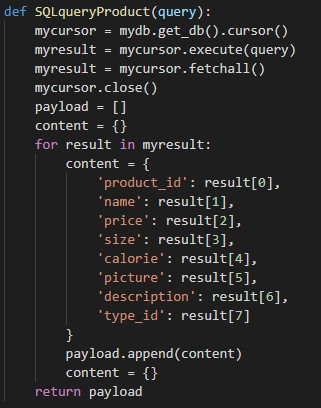
\includegraphics[width=0.5\textwidth]{drinks_1.jpg}
\caption{Funkcija, ki prebere podatke iz podatkovne baze}
\label{Drinks_DB_function}
\end{center}
\end{figure}

\begin{figure}[!htb]
\begin{center}
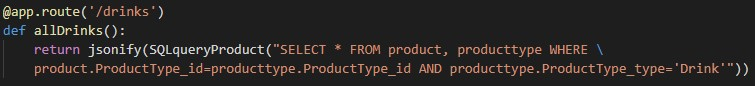
\includegraphics[width=14cm]{drinks_2.jpg}
\caption{Funkcija, ki na relativno stran \textit{drinks} servira podatke}
\label{Drinks_URI}
\end{center}
\end{figure}

Tako smo dobili vmesnik, ki na zahtevo odjemalca odgovori s podatki v formatu JSON. Na sliki~\ref{ServerEX} je primer zahtevka v programu Postman, ko odjemalec zahteva podatke vseh pijač iz podatkovne baze (metoda GET protokola HTTP). Strežnik omogoča tudi sprejemanje podatkov z metodami PUT in POST. Mi smo uporabili metodo POST za posredovanje podatkov, ki so potrebnih za zapis v podatkovno bazo, na strežnik. Spremljanje zahtevkov na strani strežnika je mogoče v konzolnem vmesniku CLI, ki se uporablja pri zagonu strežnika, slika~\ref{ServerEX2}.

\begin{figure}[!htb]   
\begin{center}
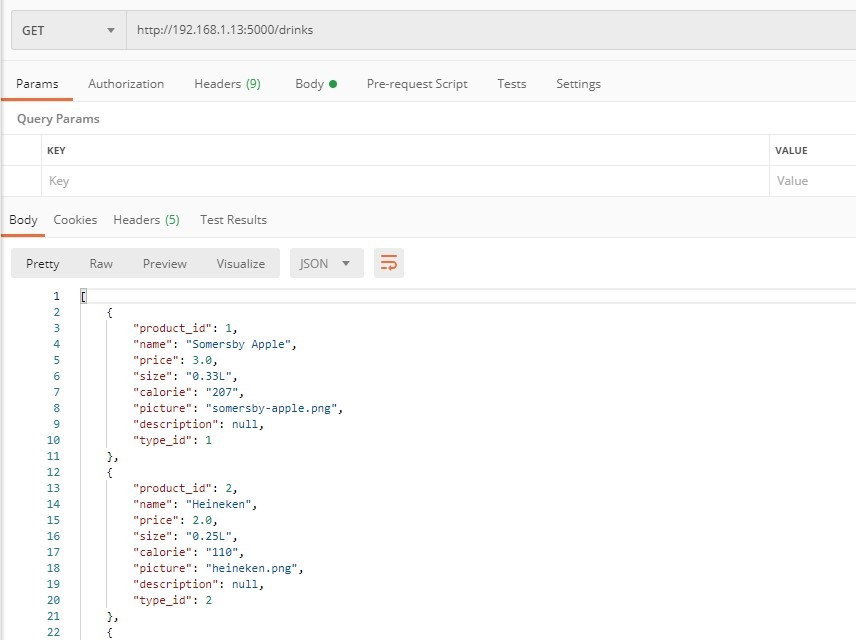
\includegraphics[width=10cm]{Server_example.jpg}
\caption{Primer serviranja podatkov na strežniku s programom Postman}
\label{ServerEX}
\end{center}
\end{figure}

\begin{figure}[!htb]
\begin{center}
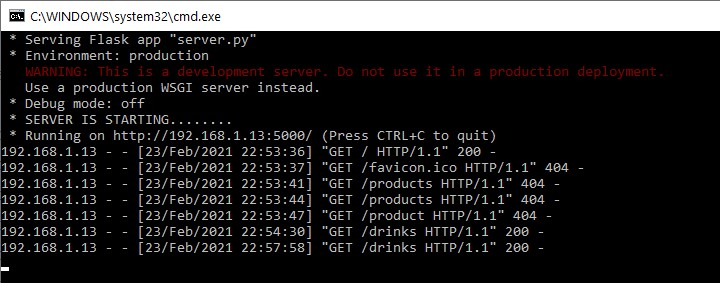
\includegraphics[width=12cm]{Server_example_2.jpg}
\caption{Primer spremljanja zahtevkov, ki prihajajo na strežnik}
\label{ServerEX2}
\end{center}
\end{figure}

Za potrebe pridobivanja podatkov v realnem času na strani odjemalca, smo potrebovali še spletni vtičnik SocketIO. Implementirali smo ga na strani strežnika in odjemalca. Zagotavlja dvosmerno komunikacijo oziroma komunikacijo na podlagi dogodkov. Deluje na vseh platformah, brskalnikih ali napravah. Uporabili smo ga zaradi medsebojnega obveščanja odjemalcov o spremembah v podatkovni bazi. Uporabili smo funkcijo \textit{emit}, ki omogoča dodajanje podatkov in izbiranje načina razpršenega oddajanja (ang. broadcast). To pomeni, da vsi prejemajo te informacije ob oddajanju na strani strežnika. Gre predvsem za splošne podatke, tako da ne more priti do zlorabe. Npr. ob spremembi naročila na strani gosta se te razlike preverijo na strežniku in vpišejo v podatkovno bazo ter o tem obvesti natakarja s funkcijo \textit{emit}, ki vsebuje številko naročila v katerem je prišlo do sprememb. 
	

Aplikacija omogoča urejanje določenih podatkov, zato smo morali zagotoviti ustrezno varnost za urejanje le-teh. Prvi nivo varnosti je avtorizacija odjemalca. Zahtevki, ki se pošiljajo na strežnik morajo biti omogočeni samo avtoriziranim odjemalcem. Zato smo uporabili HTTP piškotke (ang. cookies), ki so izdelani za spletne brskalnike in so namenjeni za sledenje, prilagajanje in shranjevanje informacij o posamezni seji uporabnika. Vsi piškotki so shranjeni na strani odjemalca in so kriptografsko zaščiteni pred morebitnimi neopoblaščenimi posegi. S tem odjemalcu preprečujemo spreminjanje podatkov v piškotkih oz. lahko nedovoljene spremembe podatkov na strežniku zaznamo. Uporabili smo Flask-Login, ki omogoča vse funkcionalnost za upravljanje uporabniških sej. 
Na sliki~\ref{Cookies} je prikazano delovanje HTTP piškotkov. Strežnik ob prvem zahtevku, torej ob uspešni prijavi, odjemalcu vrne piškotek. Odjemalec ob vsakem nadaljnjem zahtevku doda piškotek s katerim strežnik overi zahtevo odjemalca.

\begin{figure}[!htb]
\begin{center}
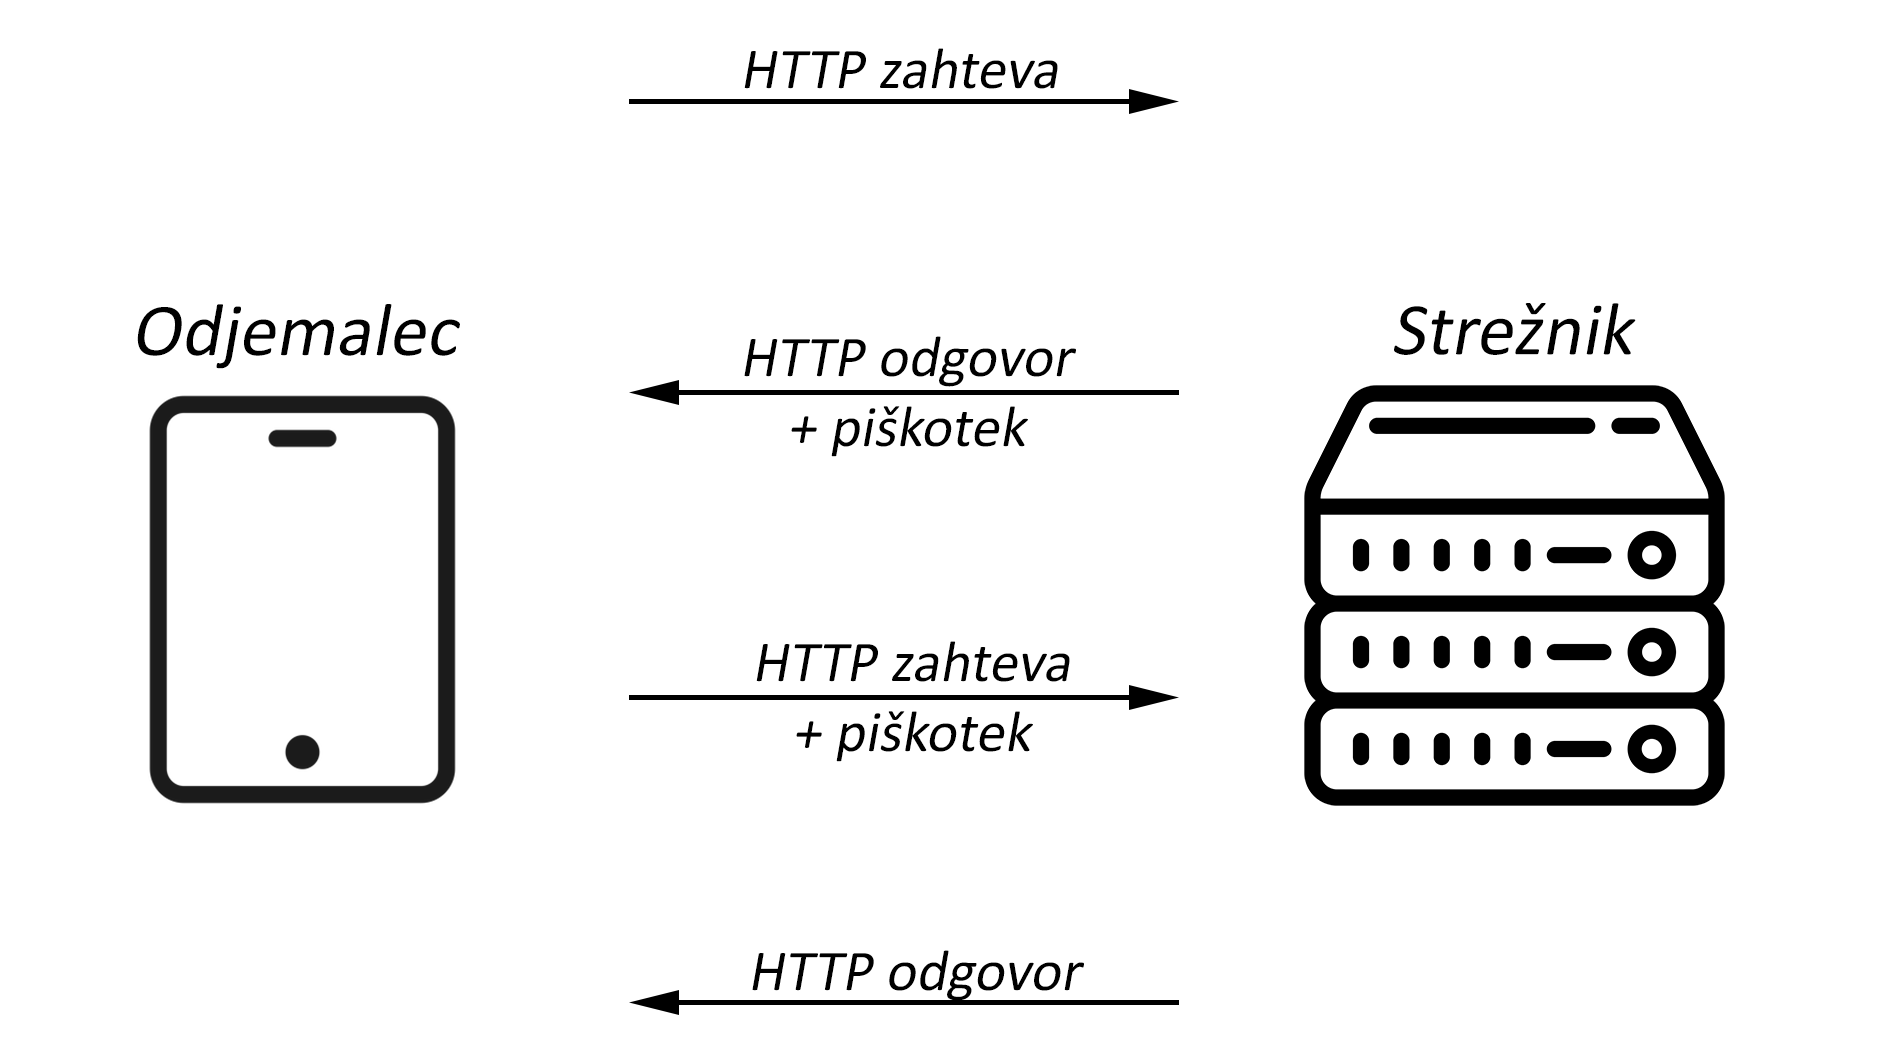
\includegraphics[width=14cm]{cookie-how1.png}
\caption{Delovanje HTTP piškotkov med odjemalcem in strežnikom}
\label{Cookies}
\end{center}
\end{figure}

\section{Odjemalec}

Odjemalca bi lahko implementirali v spletnih tehnologijah (HTML, CSS in JavaScript) ali pa v namenski mobilni aplikaciji. Odločili smo se za spletne tehnologije, kjer je glavnina odjemalca implementrana v programskem jeziku JavaScript s pomočjo ogrodja Vue	.  Naredili smo odziven in reaktiven vmesnik, ki deluje v realnem času. Vue je eden izmed mnogih kot npr. Angular, Ember, React,… poznan pa je predvsem zaradi enostavnosti za upravljanje in izvajanje testov. Vsem je skupna reaktivnost, vendar v drugačnem pomenu besede. Reaktivnost \cite{reaktivnost}, je programska paradigma, ki nam omogoča, da se na deklarativni način prilagodimo spremembam. Tako deluje tudi reaktivnost v aplikacijah za razliko, da je podatek lahko vezan na več funkciji oziroma delov programske kode, ki se ob spremembi vrednosti posodobijo. Vue je namenjen izdelavi projektov SPA (ang. single-page application), saj vsebuje samo eno datoteko HTML. To prednost smo izkoristili s pomočjo ostalih knjižnic, ki so nam olajšale izdelavo aplikacije. Uporabili smo naslednje:
\begin{description}
\item[Vue CLI] velja kot standardno orodje za ekosistem Vue \cite{VueCLI}. Zagotavlja, da že pri gradnji novega projekta poveže različne dodatke med seboj. To omogoča razviljacu, da se bolj osredotoči na programiranje in ne na povezovanje njih v projekt. Z uporabo vmesnika CLI se lahko izbere projekt, kjer so na voljo že privzete nastavitve, lahko pa se jih tudi nastavi po meri. Mi smo uporabili Vuex, Vue-Router, ESLint in Vuetify.
\item[Vuex] je knjižnica za shranjevanje vrednosti v aplikacijah Vue.js \cite{Vuex}. Služi kot centralizirana baza podatkov za vse komponente v aplikaciji. 
\item[Vue-Router] je uradni usmerjevalnik za Vue.js \cite{VueRouter}. Integrira se globoko z jedrom Vue.js, tako da poenostavi izdelavo SPA aplikacij. Usmerjevalnik je mišljen v smislu usmerjanja na druge komponente (angl. Component), ki v Vue.js predstavljajo druge poglede, lahko bi rekli podobno kot podstrani.
\item[ESLint] je orodje za prepoznavanje in poročanje o popravkih v programski kodi \cite{ESLint}. Cilj je narediti kodo bolj pregledno in urejeno, kar pripomore k izogibanju napak.
\item[Vuetify] je eden izmed mnogih uporabniških vmesnikov, ki je zgrajen na vrhu Vue.js \cite{Vuetify}. Za razliko od drugih vmesnikov je Vuetify enostaven za učenje z več stotimi komponentami izdelanih po specifikacijah Material Design.
\item[Vue-devtools] je zgolj dodatek v brskalniku, ki omogoča lažje sledenje delovanja aplikacije in detektiranju napak. 
\end{description}


Programsko izvedbo na strani odjemalca smo razdelili v tri vloge oziroma dve aplikaciji. Ena aplikacija je namenjena natakarjem in kuharjem, ki se ločuje s prijavnim oknom in izgledom vmesnika. Druga aplikacija je namenjena samo gostom ter je sestavljena iz več pogledov. Ločili smo jih zaradi varnosti, lažjega razvijanja in preglednosti, saj gre za dve popolnoma različni aplikaciji. Vse funkcionalnosti in delovanje ene in druge aplikacije so opisane v naslednjem poglavju. Sliki~\ref{Gost} in~\ref{NatakarGost} prikazujeti izgled obeh aplikacij.

\begin{figure}[!htb]
\begin{center}
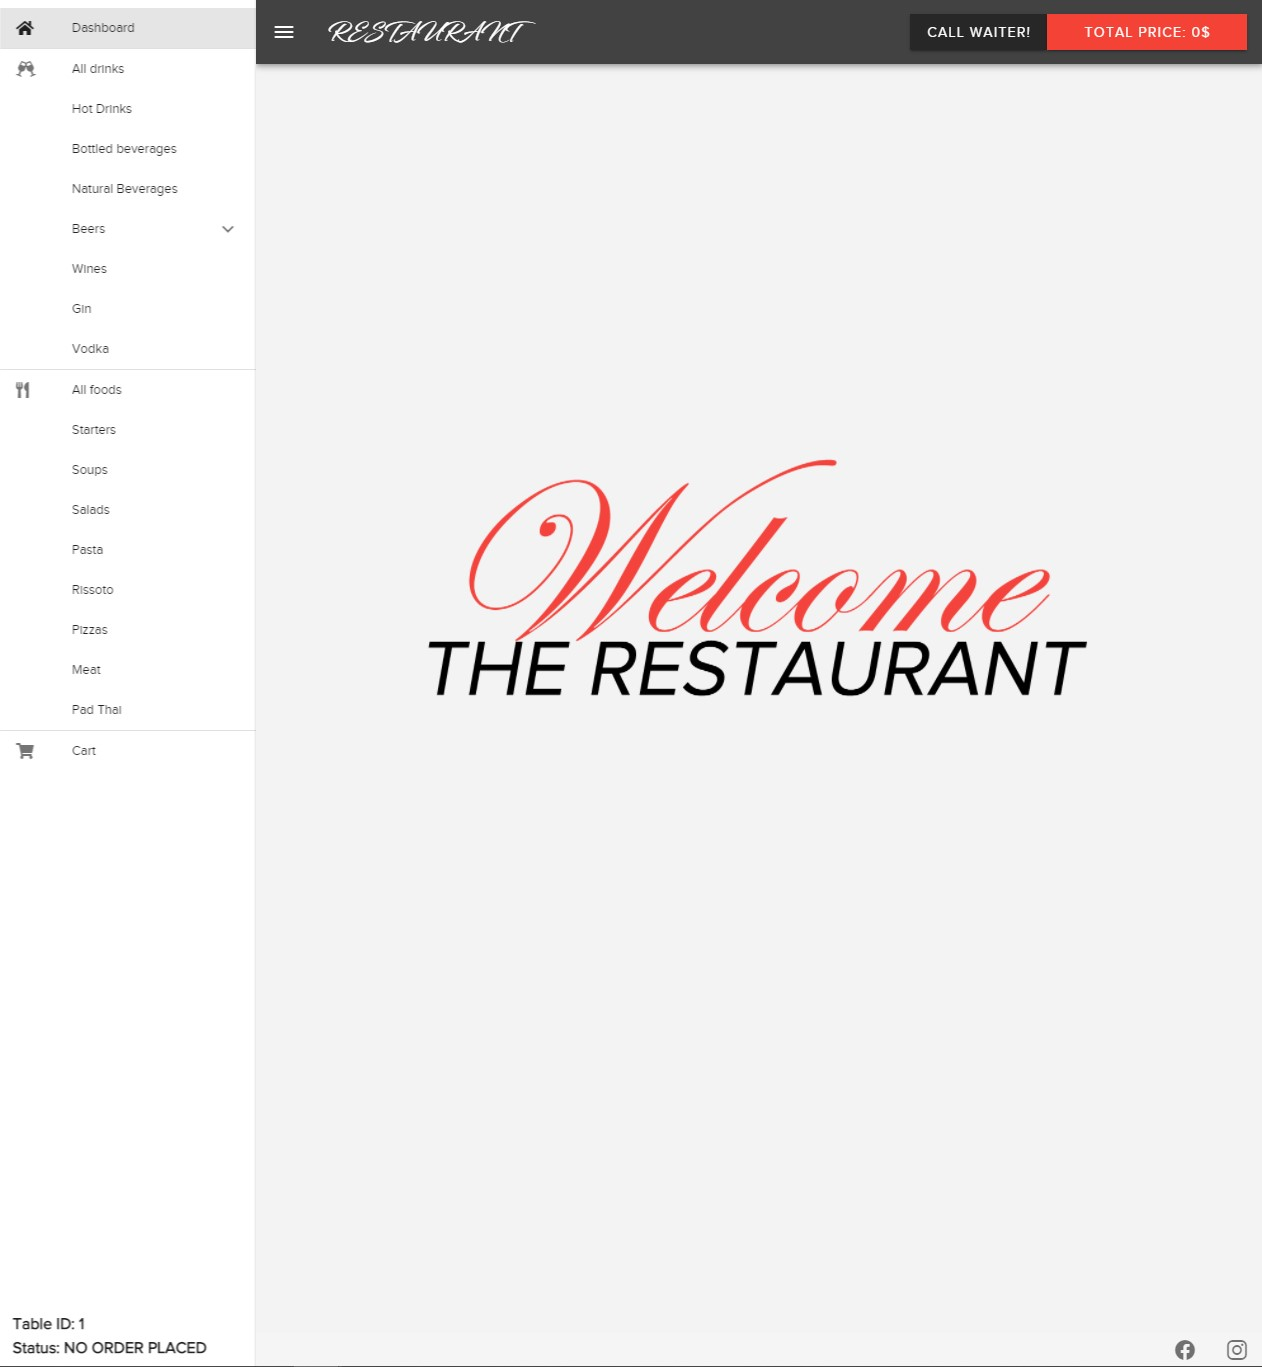
\includegraphics[width=12cm]{gost_1.jpg}
\caption{Spletni vmesnik za gosta}
\label{Gost}
\end{center}
\end{figure}

\begin{figure}[!htb]
\begin{center}
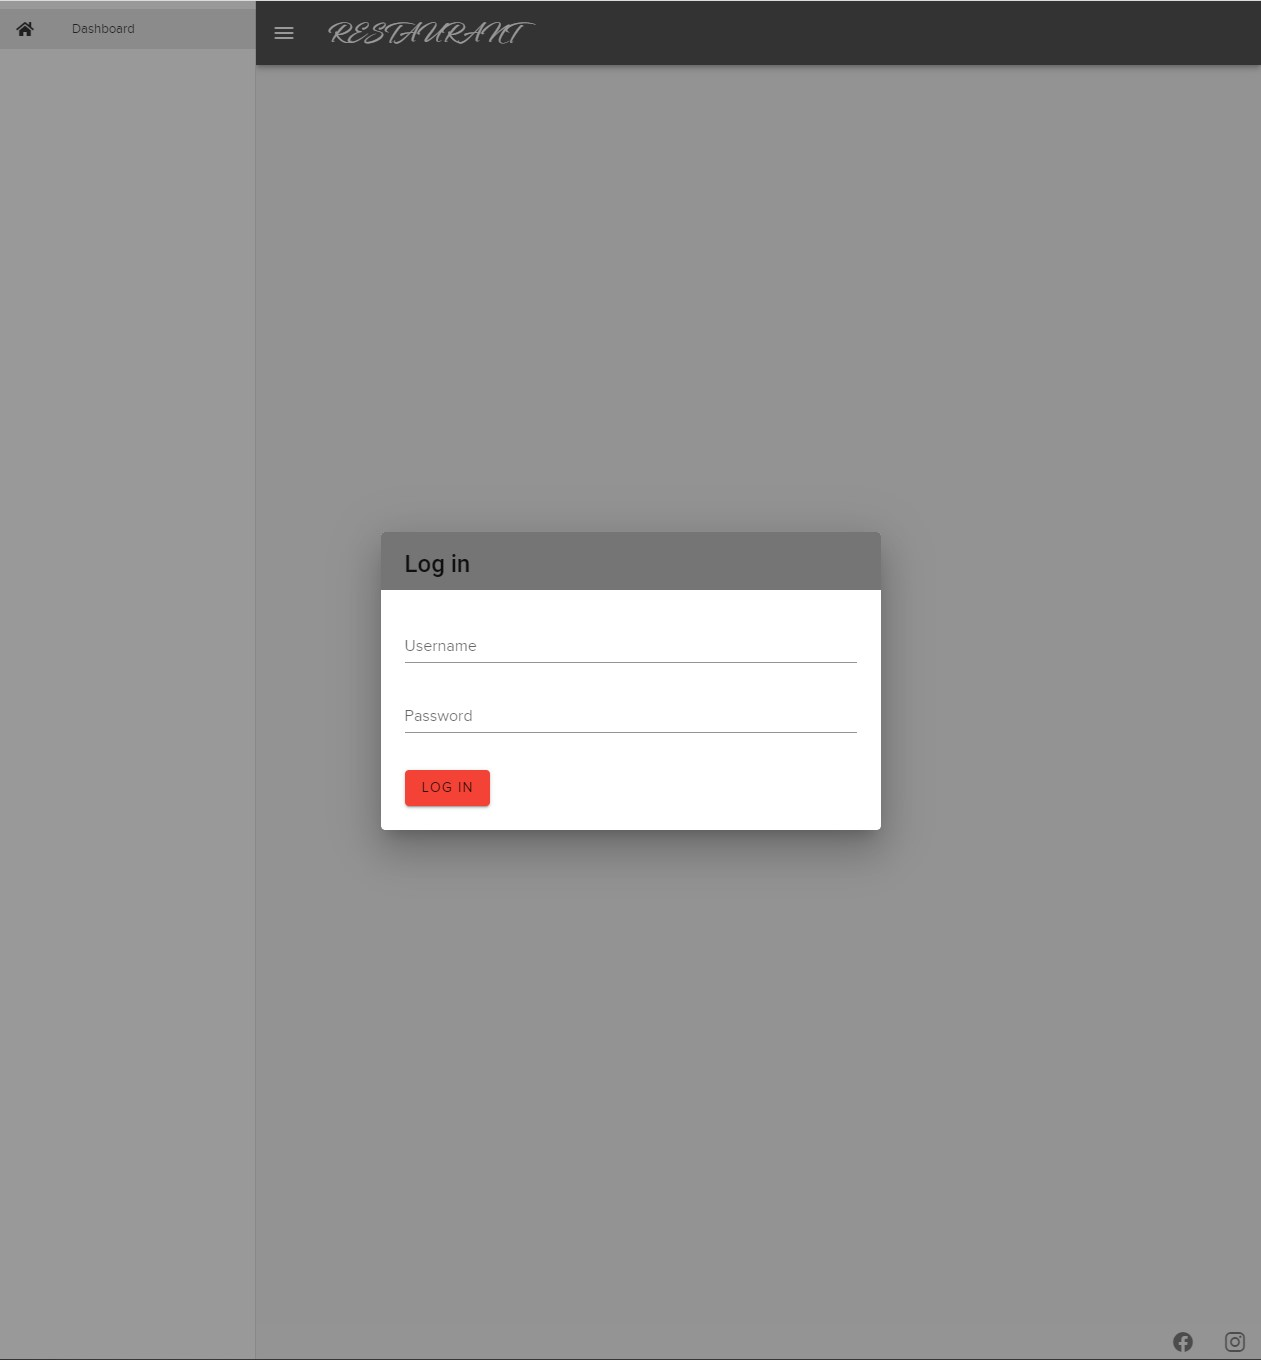
\includegraphics[width=12cm]{natakar-gost_1.jpg}
\caption{Spetni vmesnik za natakarja in kuharja}
\label{NatakarGost}
\end{center}
\end{figure}

Ena izmed pomembnih stvari pri obratovanje restavracije je čim hitrejša postrežba katero je mogoče izboljšati s čim hitrejšo komunikacijo. Zato smo, enako kot na strani strežnika, uporabili spletni vtičnik SocketIO. To smo vključili v obeh aplikacijah, in sicer za oddajanje naročil, posodabljanje naročil, obvečanju gosta o stanju naročila, itd. Najprej smo hoteli uporabiti samodejno osveževanje na določen časovni interval, vednar je uporaba spletnih vtičnikov hitrejša in učinkovitejša. Slika~\ref{socketioo1} prikazuje seznam vseh vtičnikov, ki so uporabljeni na strani gosta.

\begin{figure}[!htb]
\begin{center}

\includegraphics[width=11cm]{socketio_1.jpg}
\caption{Seznam vtičnikov, ki so uporabljeni na strani gosta}
\label{socketioo1}
\end{center}
\end{figure}

Za pridobivanje podatkov na strani odjemalca smo uporabili Axios, ki je namenjen procesiranju zahtevkov  HTTP. To pomeni, da podatke, ki se oglašujejo na strani strežnika s pomočjo te knižnjice pridobimo na stran odjemalca (slika~\ref{axios_1}). 

\begin{figure}[!htb]
\begin{center}
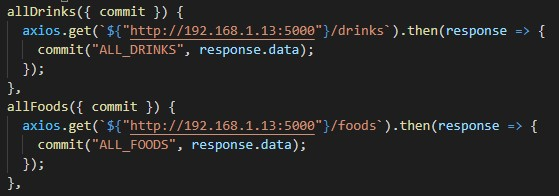
\includegraphics[width=11cm]{axios_1.jpg}
\caption{Način uporabe Axios v aplikaciji za gosta}
\label{axios_1}
\end{center}
\end{figure}


\chapter {Delovanje aplikacije}
Za prikaz delovanja smo pripravili testno okolje, kjer smo znotraj lokalnega omrežja postavili podatkovno bazo, strežnik in aplikaciji. Primer uporabe je opisan in prikazan spodaj, bolj podroben opis vseh funkcionalnosti pa v naslednjih poglavjih.

Gost s sprehajanjem skozi menije izbira hrano in pijačim ter jo sproti dodaja v naročilo (slika~\ref{Opis1}). V našem primeru gost izbere dve sokova in dve pici. Pregled naročila izvede v košarici, kjer naročilo tudi odda (slika~\ref{Opis2}).
Natakar in kuhar se prvo prijavita, da imata omogočen pregled nad naročilo. Na seznamu se jima prikaže novo naročilo, katero morata preveriti ali imata vse sestavine za pripravo (slika~\ref{Opis3}). V našem primeru naročilo vsebuje hrano, tako da mora naročilo prvo potrdi kuhar (slika~\ref{Opis4}), da lahko natakar potrdi celotno naročilo gostu (slika~\ref{Opis5}). Ko je hrana pripravljena, kuhar o tem obvesti natakarja. Natakar naročilo postreže in naročilo označi kot postreženo. Gost zaključi naročilo z zahtevanjem račun v zavihku košarica, kjer je naročilo tudi oddal. Način plačila izbere ob kliku na zahtevo (slika~\ref{Opis6}). Natakar je obveščen o zahtevi za račun in načinu plačila s strani gosta. S tiskanjem računa natakar zaključi naročilo, kar pomeni da se izbriše iz seznama aktivnih naročil.

\begin{figure}[!htb]
\begin{center}
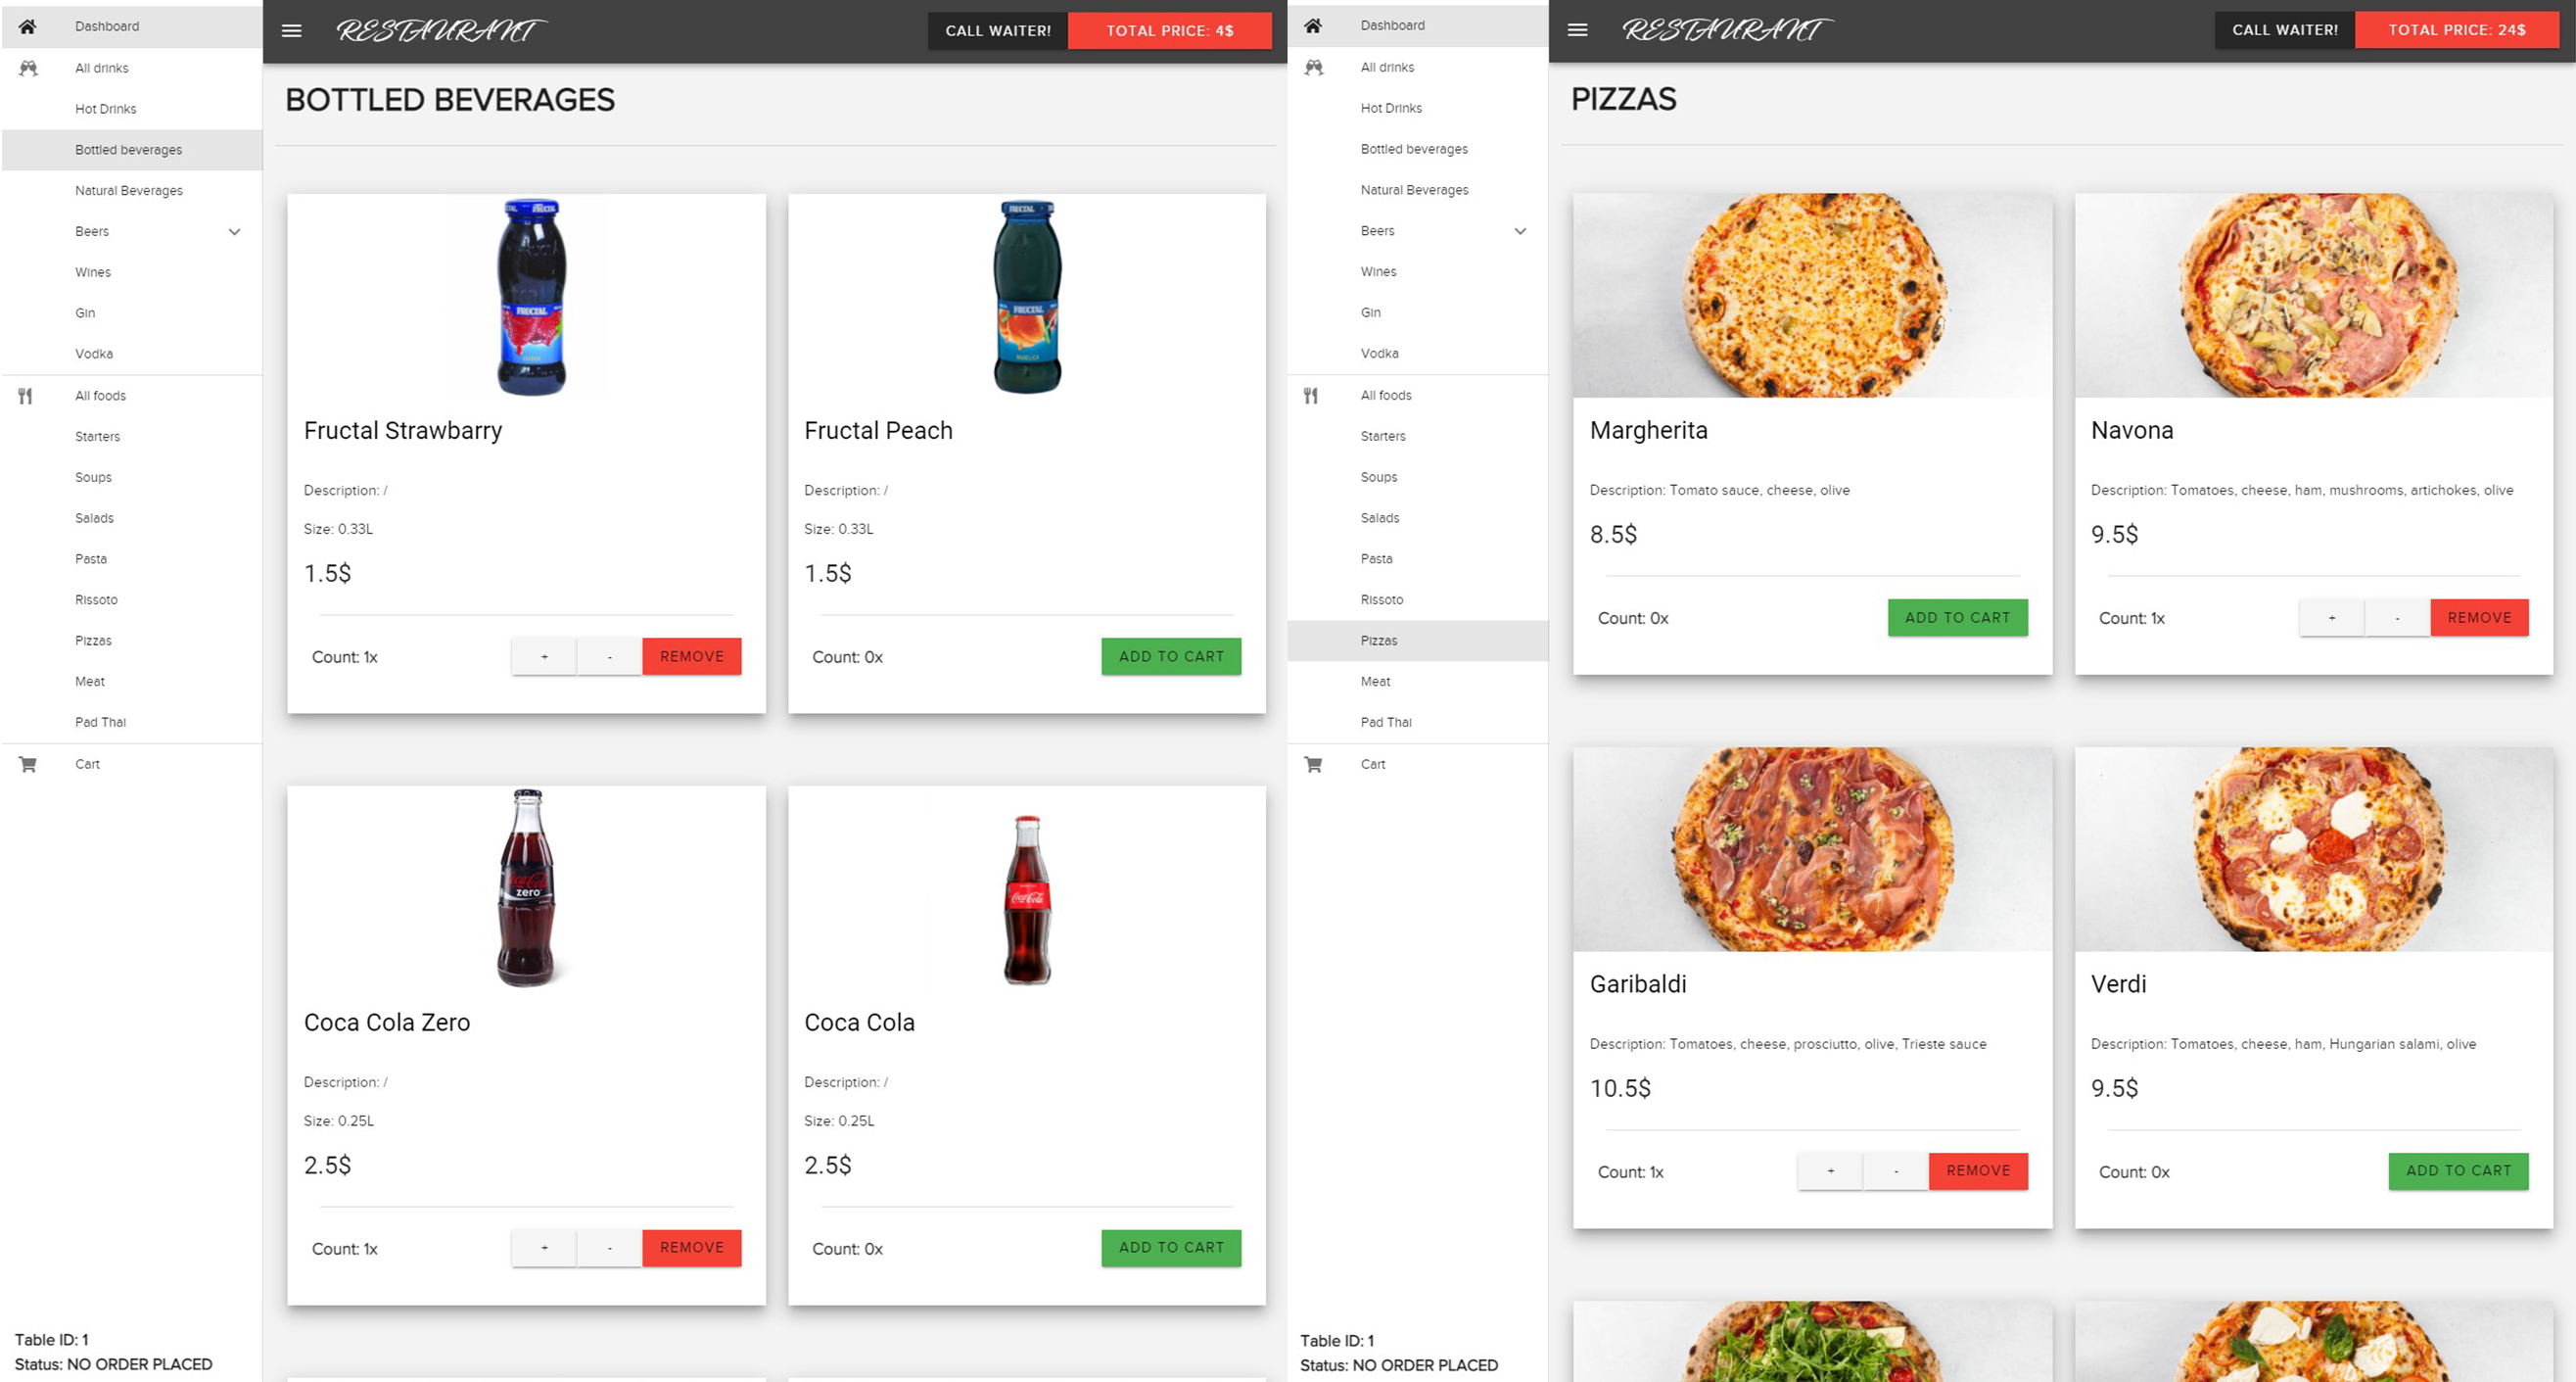
\includegraphics[width=14.5cm]{opis1.jpg}
\caption{Pregled in izbiranje hrane in pijače}
\label{Opis1}
\end{center}
\end{figure}

\begin{figure}[!htb]
\begin{center}
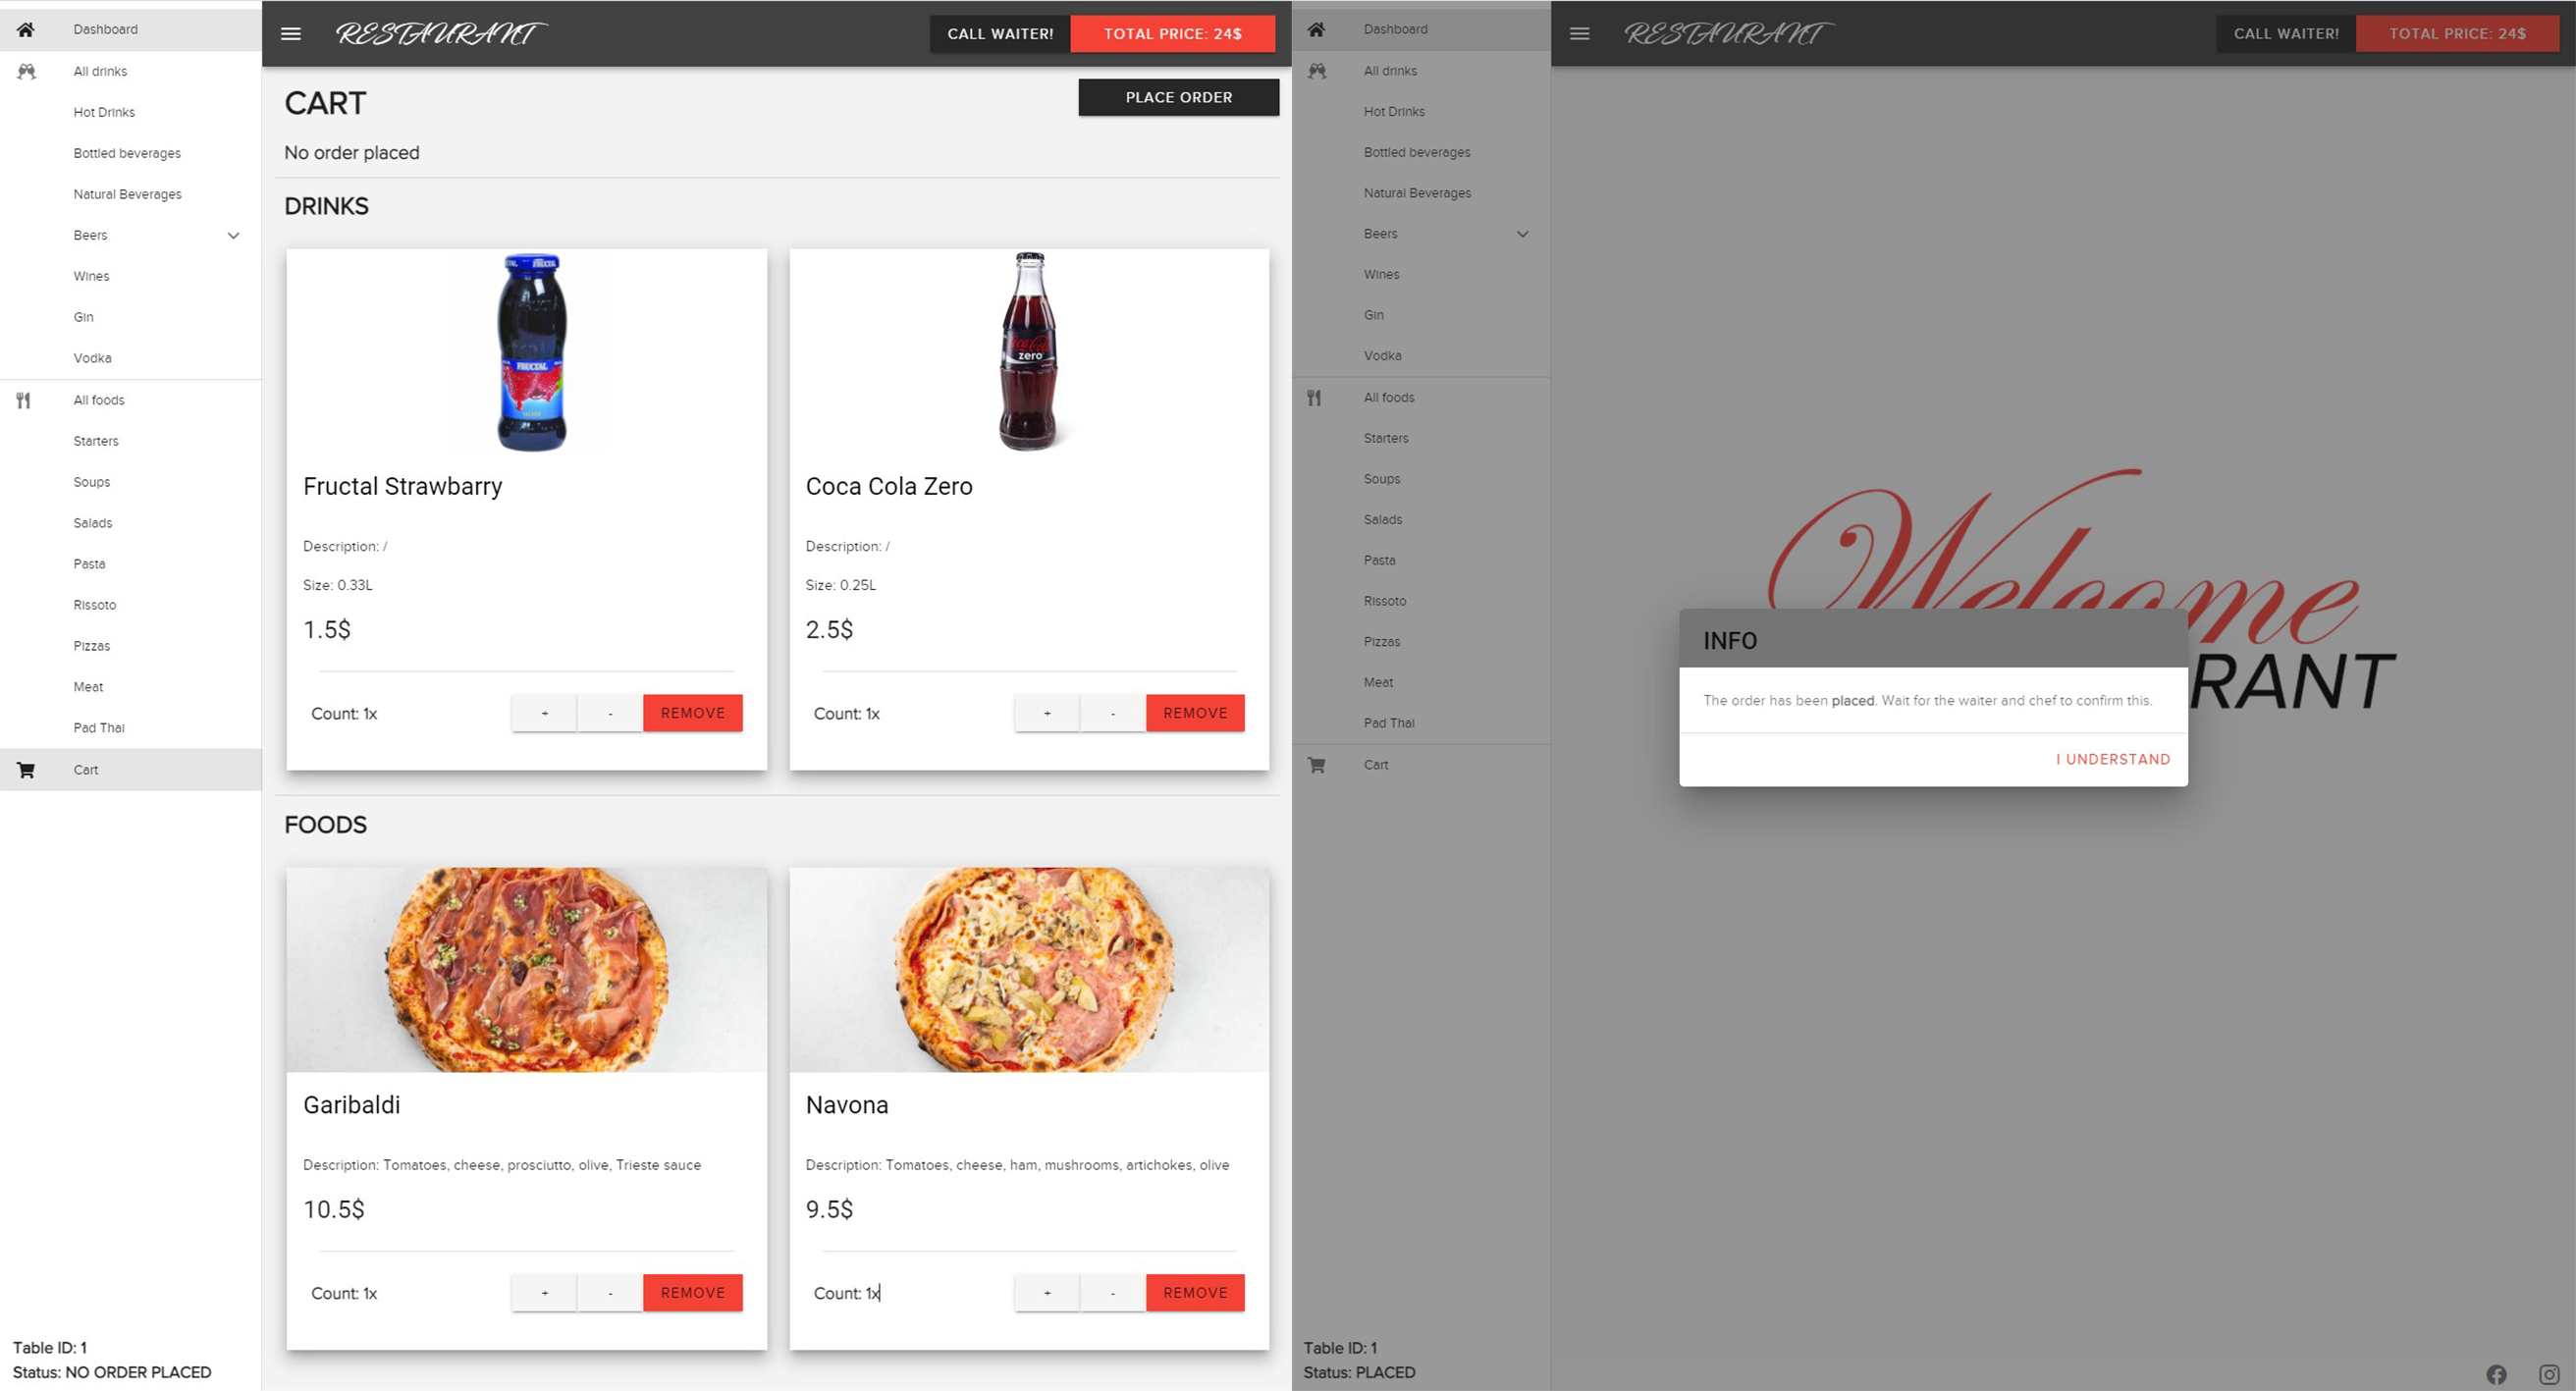
\includegraphics[width=14.5cm]{opis11.jpg}
\caption{Pregled košarice in oddajanje naročila}
\label{Opis2}
\end{center}
\end{figure}

\begin{figure}[!htb]
\begin{center}
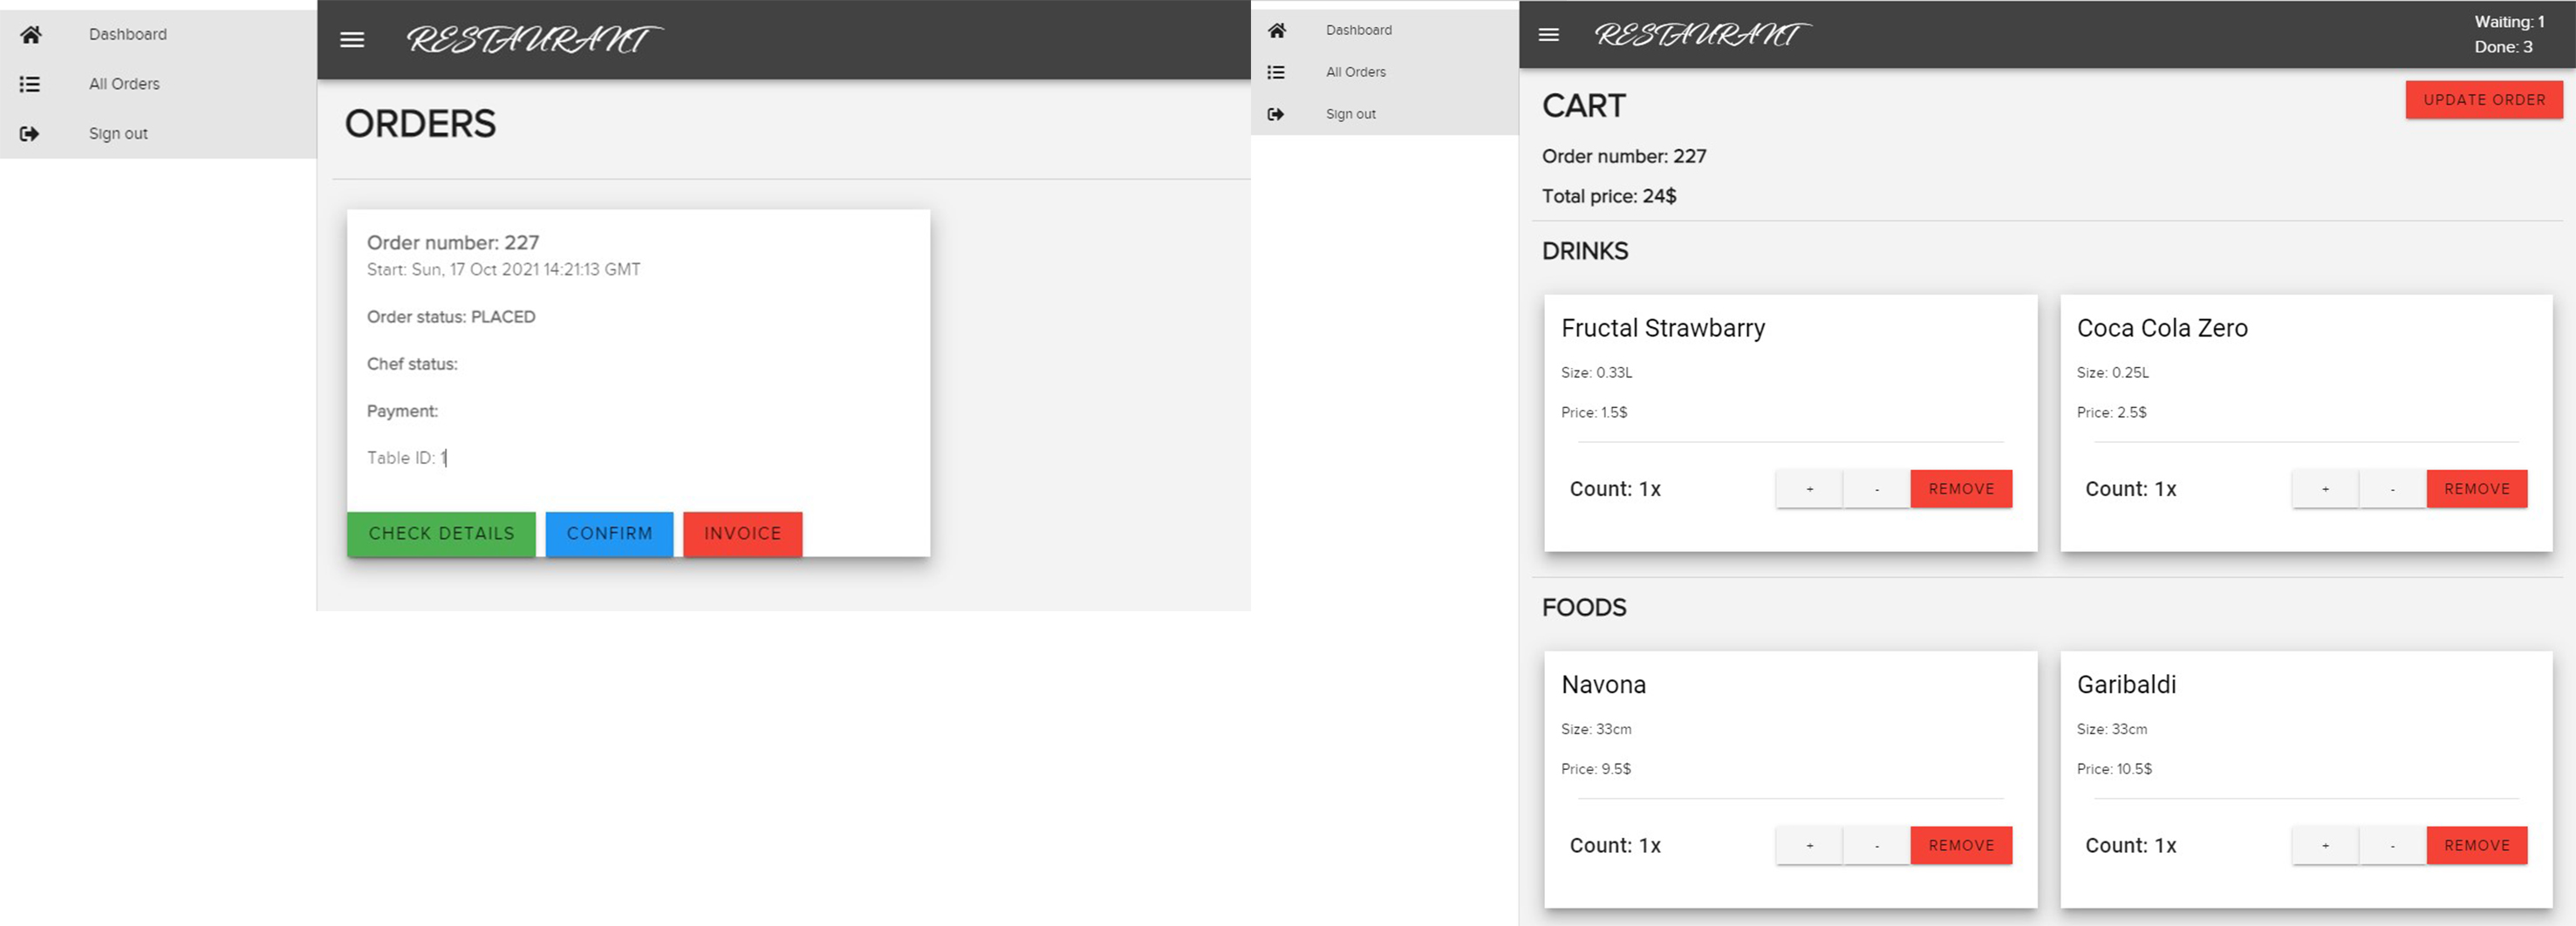
\includegraphics[width=14.5cm]{opis2.jpg}
\caption{Pregled naročila na strani natakarja}
\label{Opis3}
\end{center}
\end{figure}
	
\begin{figure}[!htb]
\begin{center}
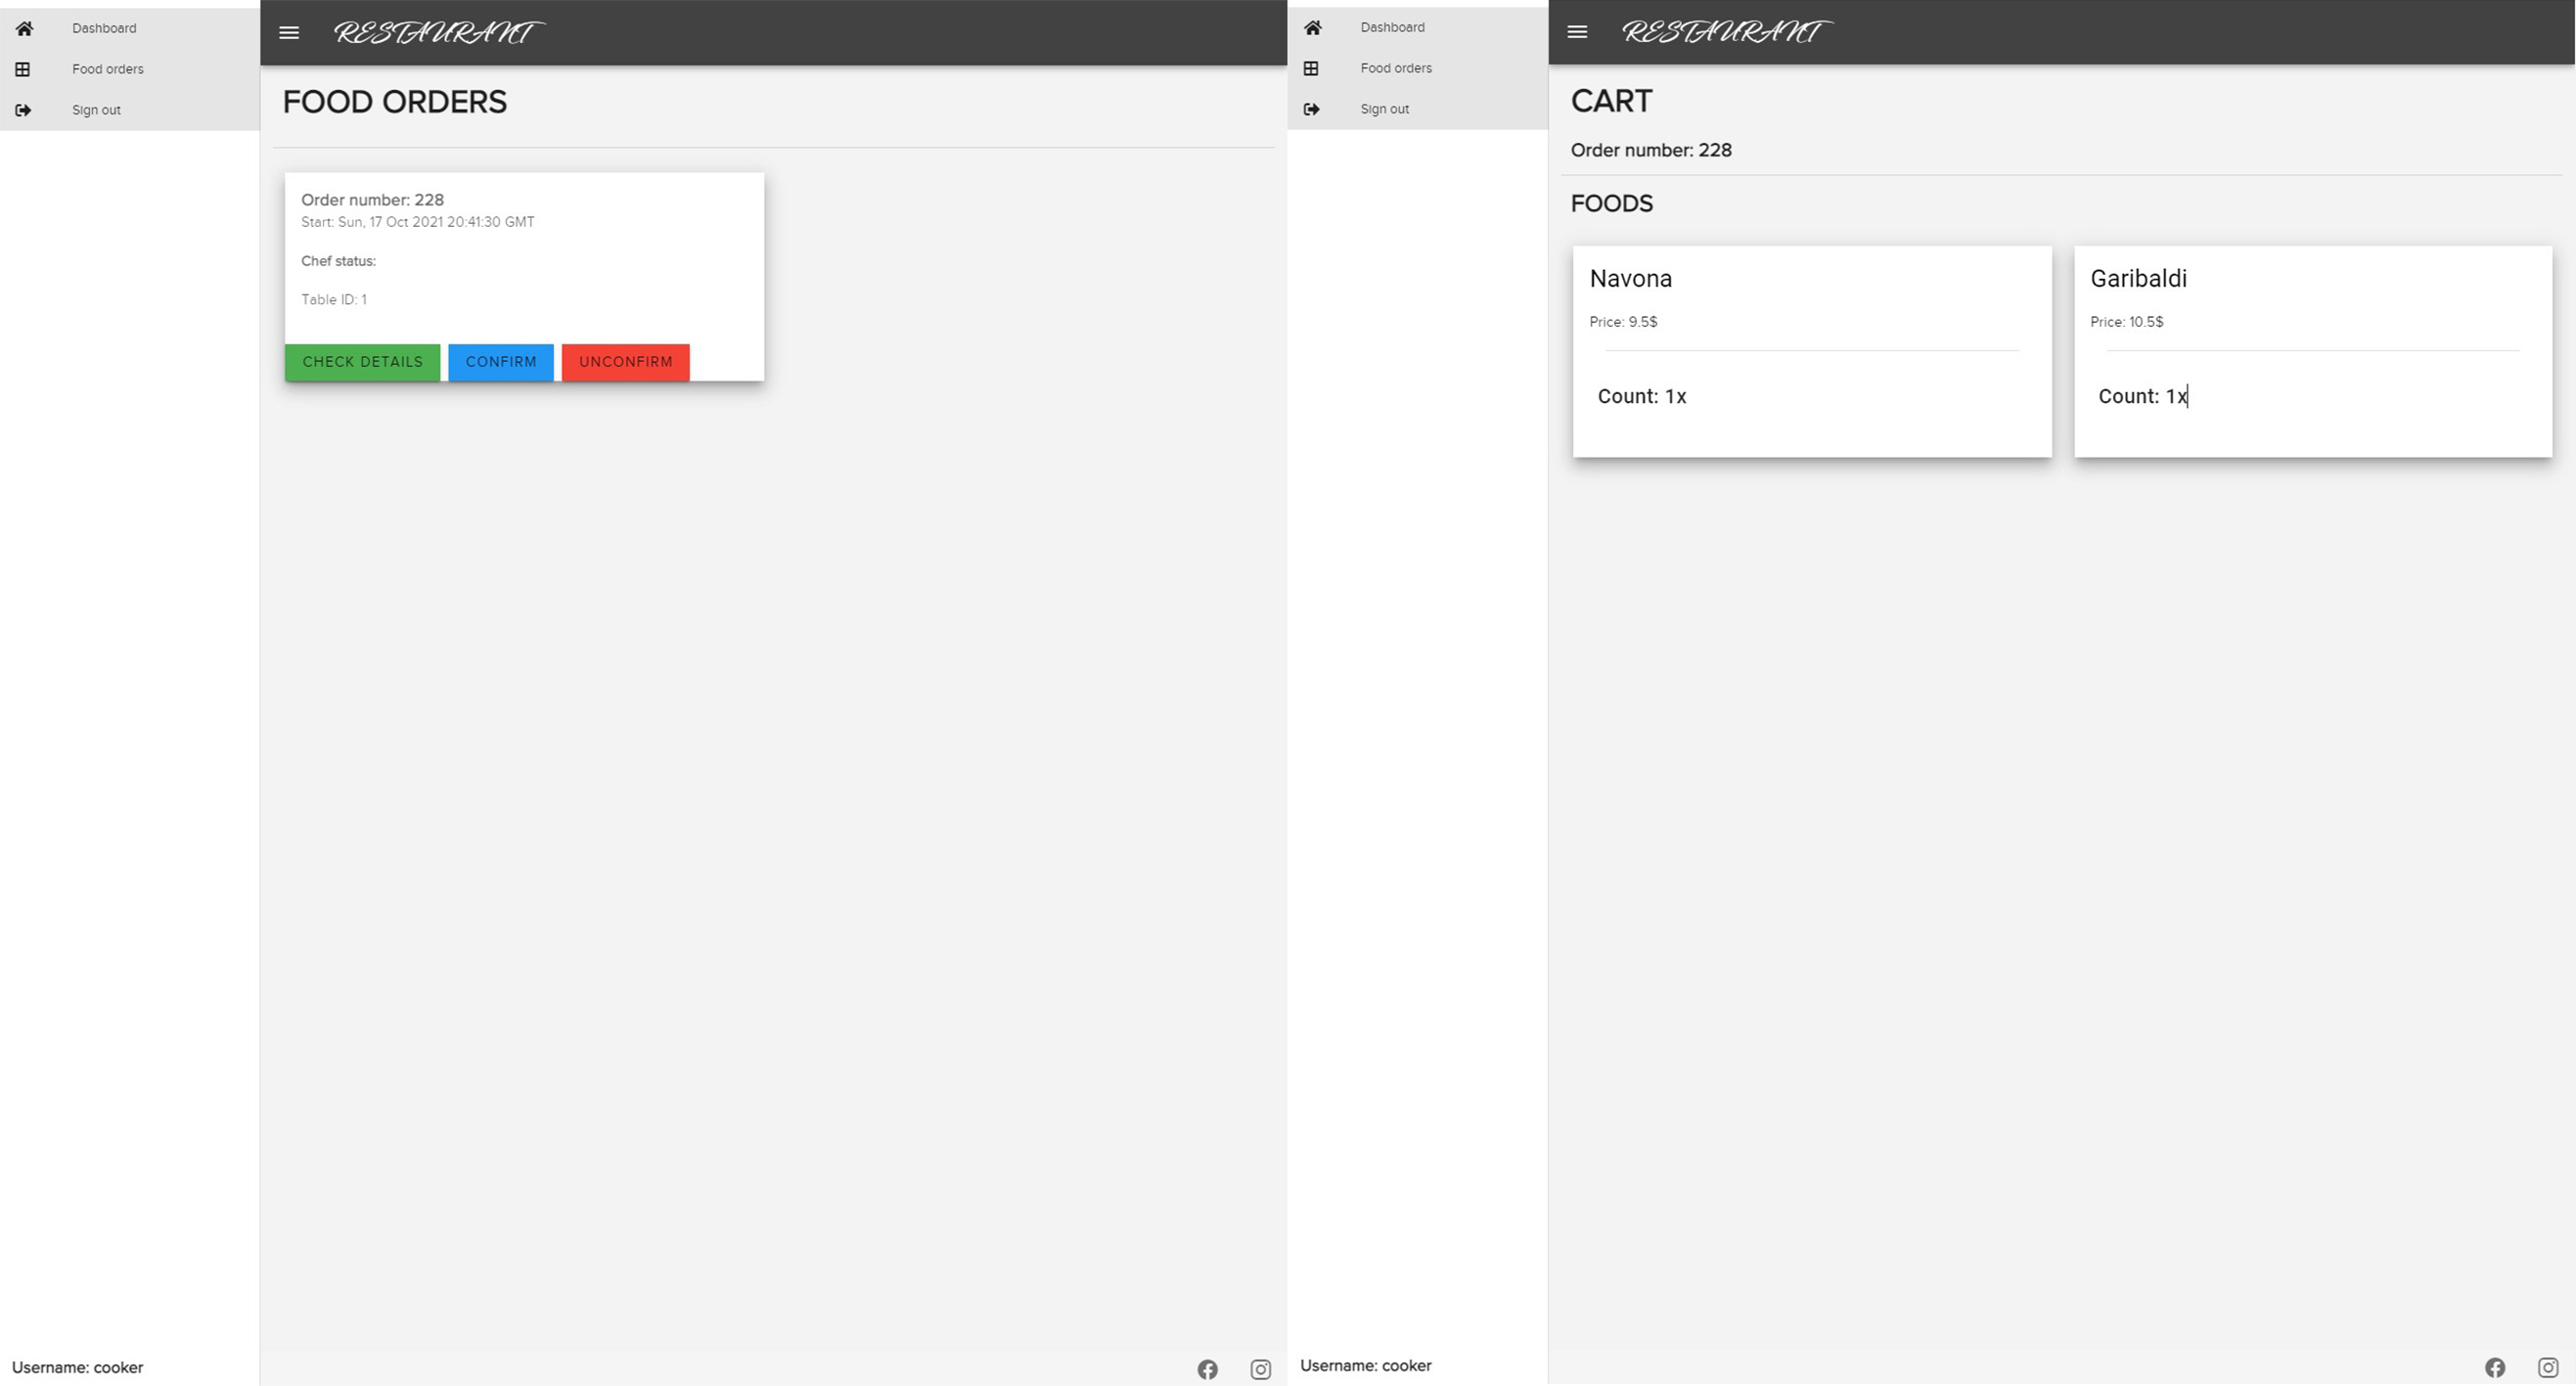
\includegraphics[width=14.5cm]{opis3.jpg}
\caption{Pregled naročila na strani kuharja}
\label{Opis4}
\end{center}
\end{figure}

\begin{figure}[!htb]
\begin{center}
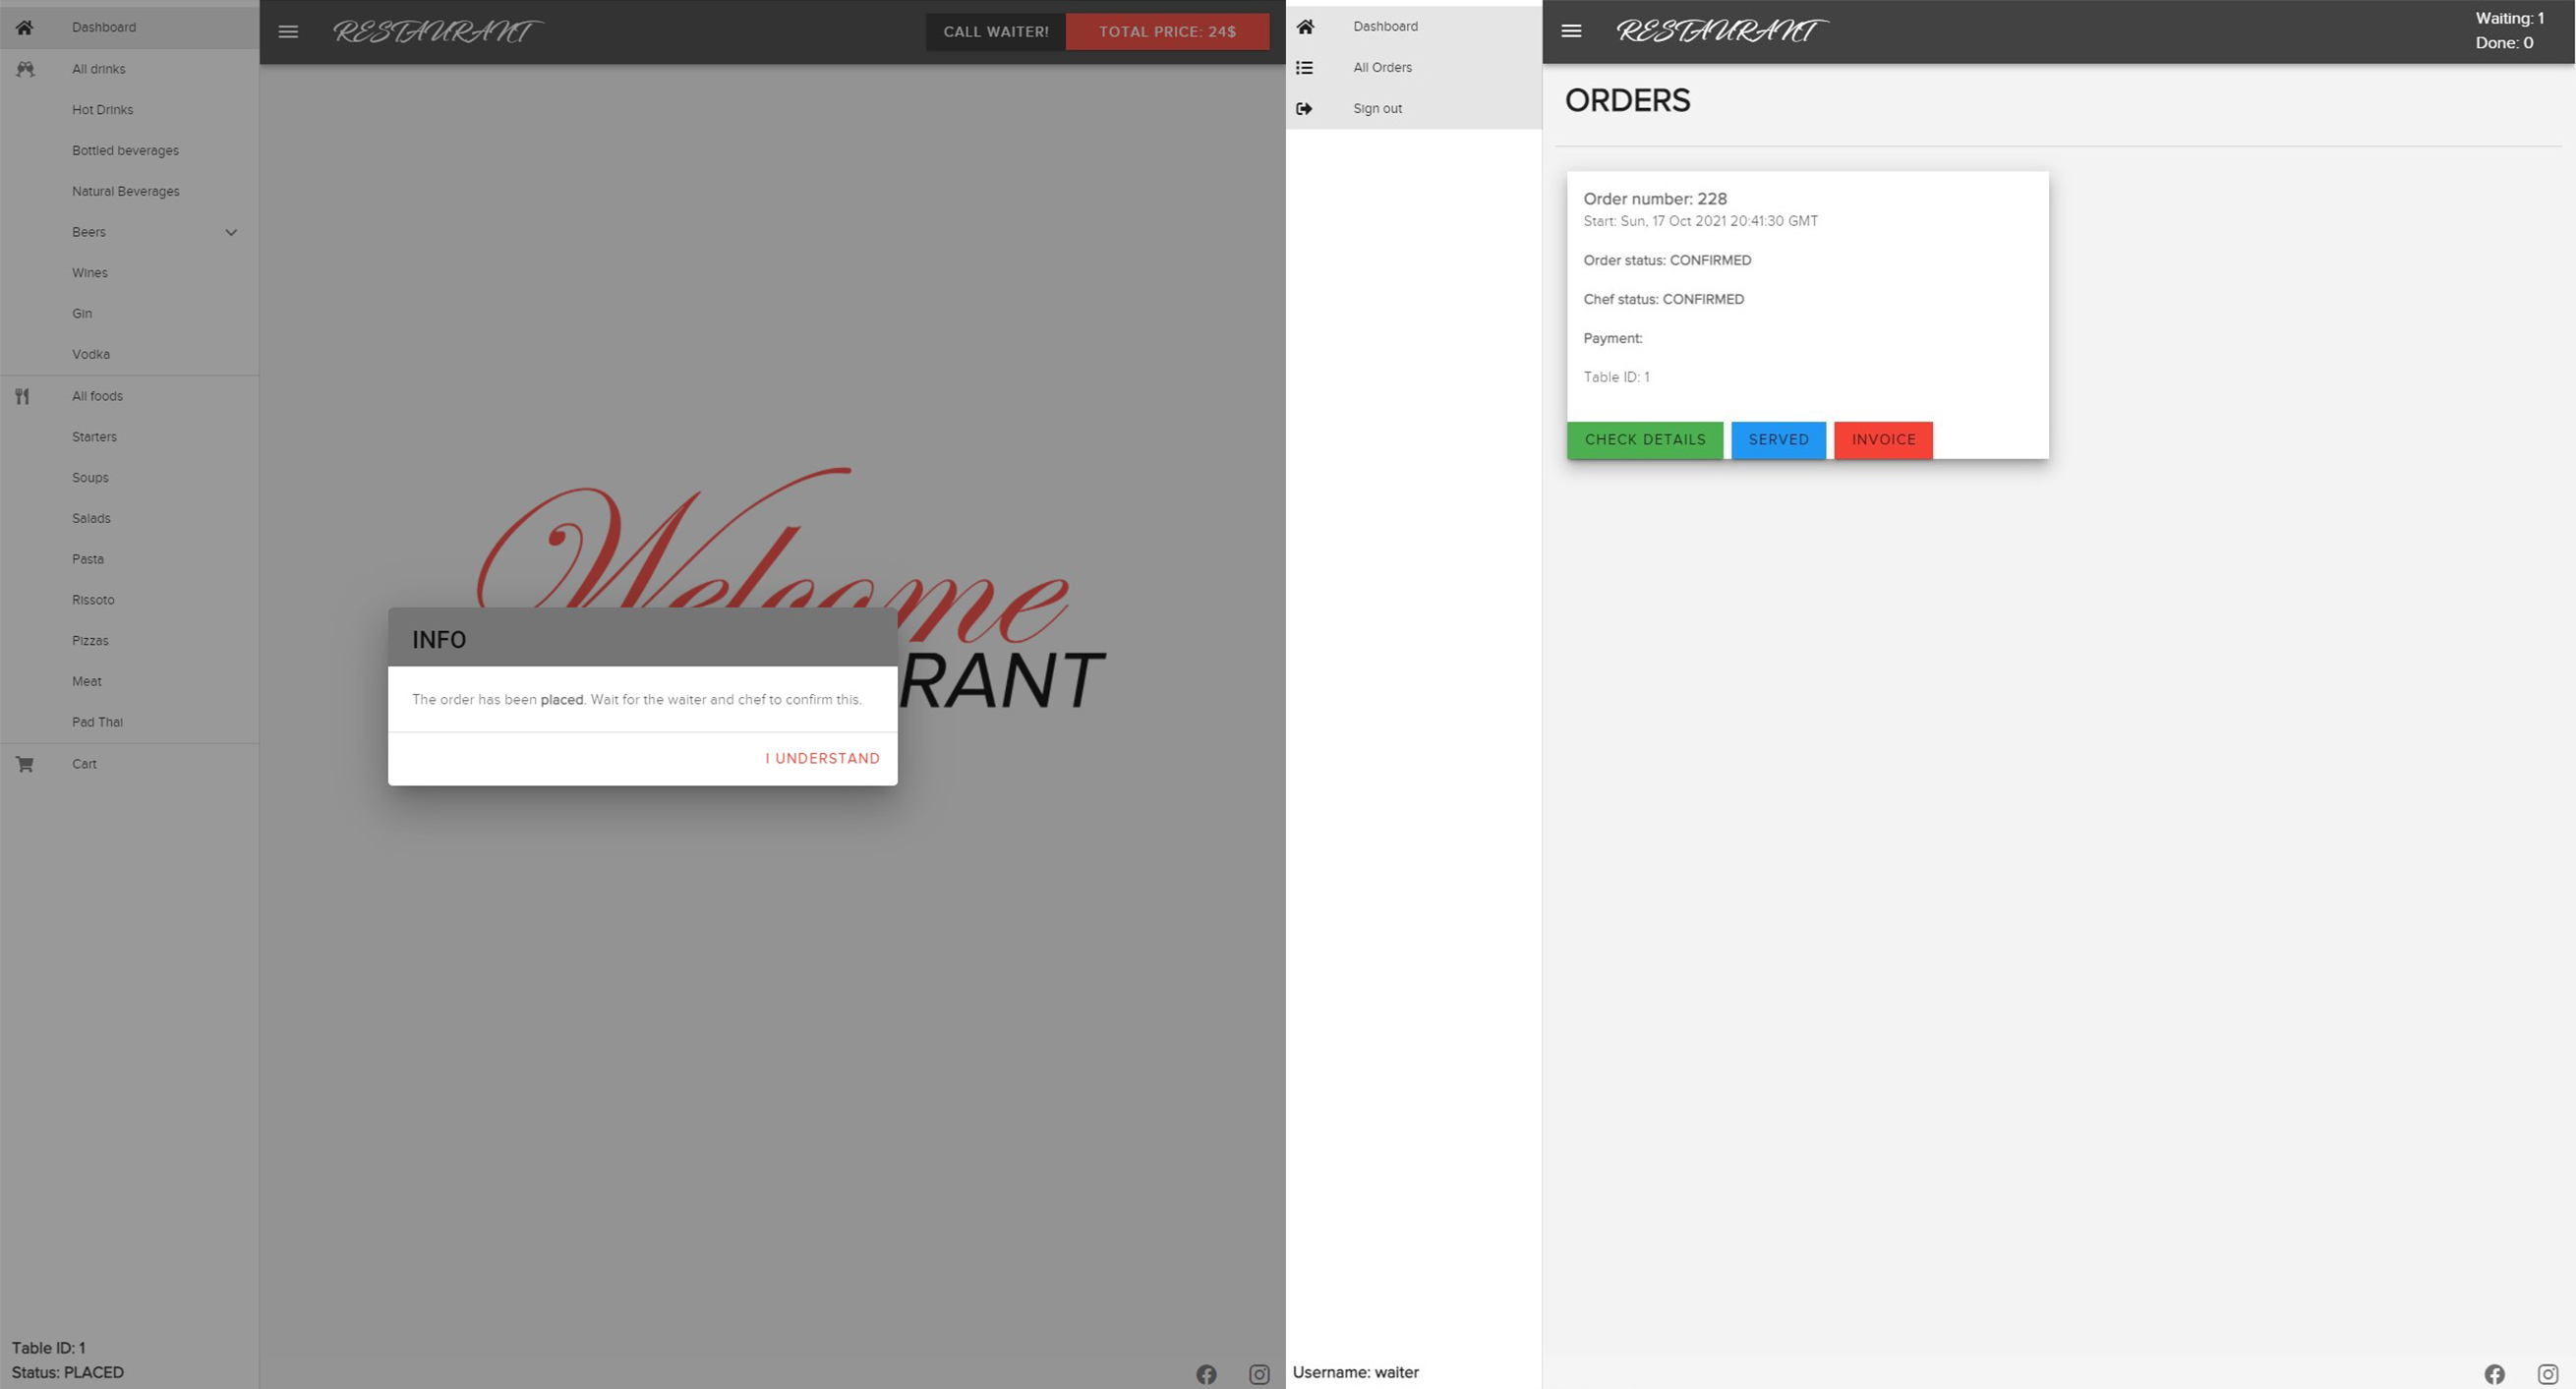
\includegraphics[width=14.5cm]{opis5.jpg}
\caption{Obveščanje gosta o sprejemu naročila}
\label{Opis5}
\end{center}
\end{figure}

\begin{figure}[!htb]
\begin{center}
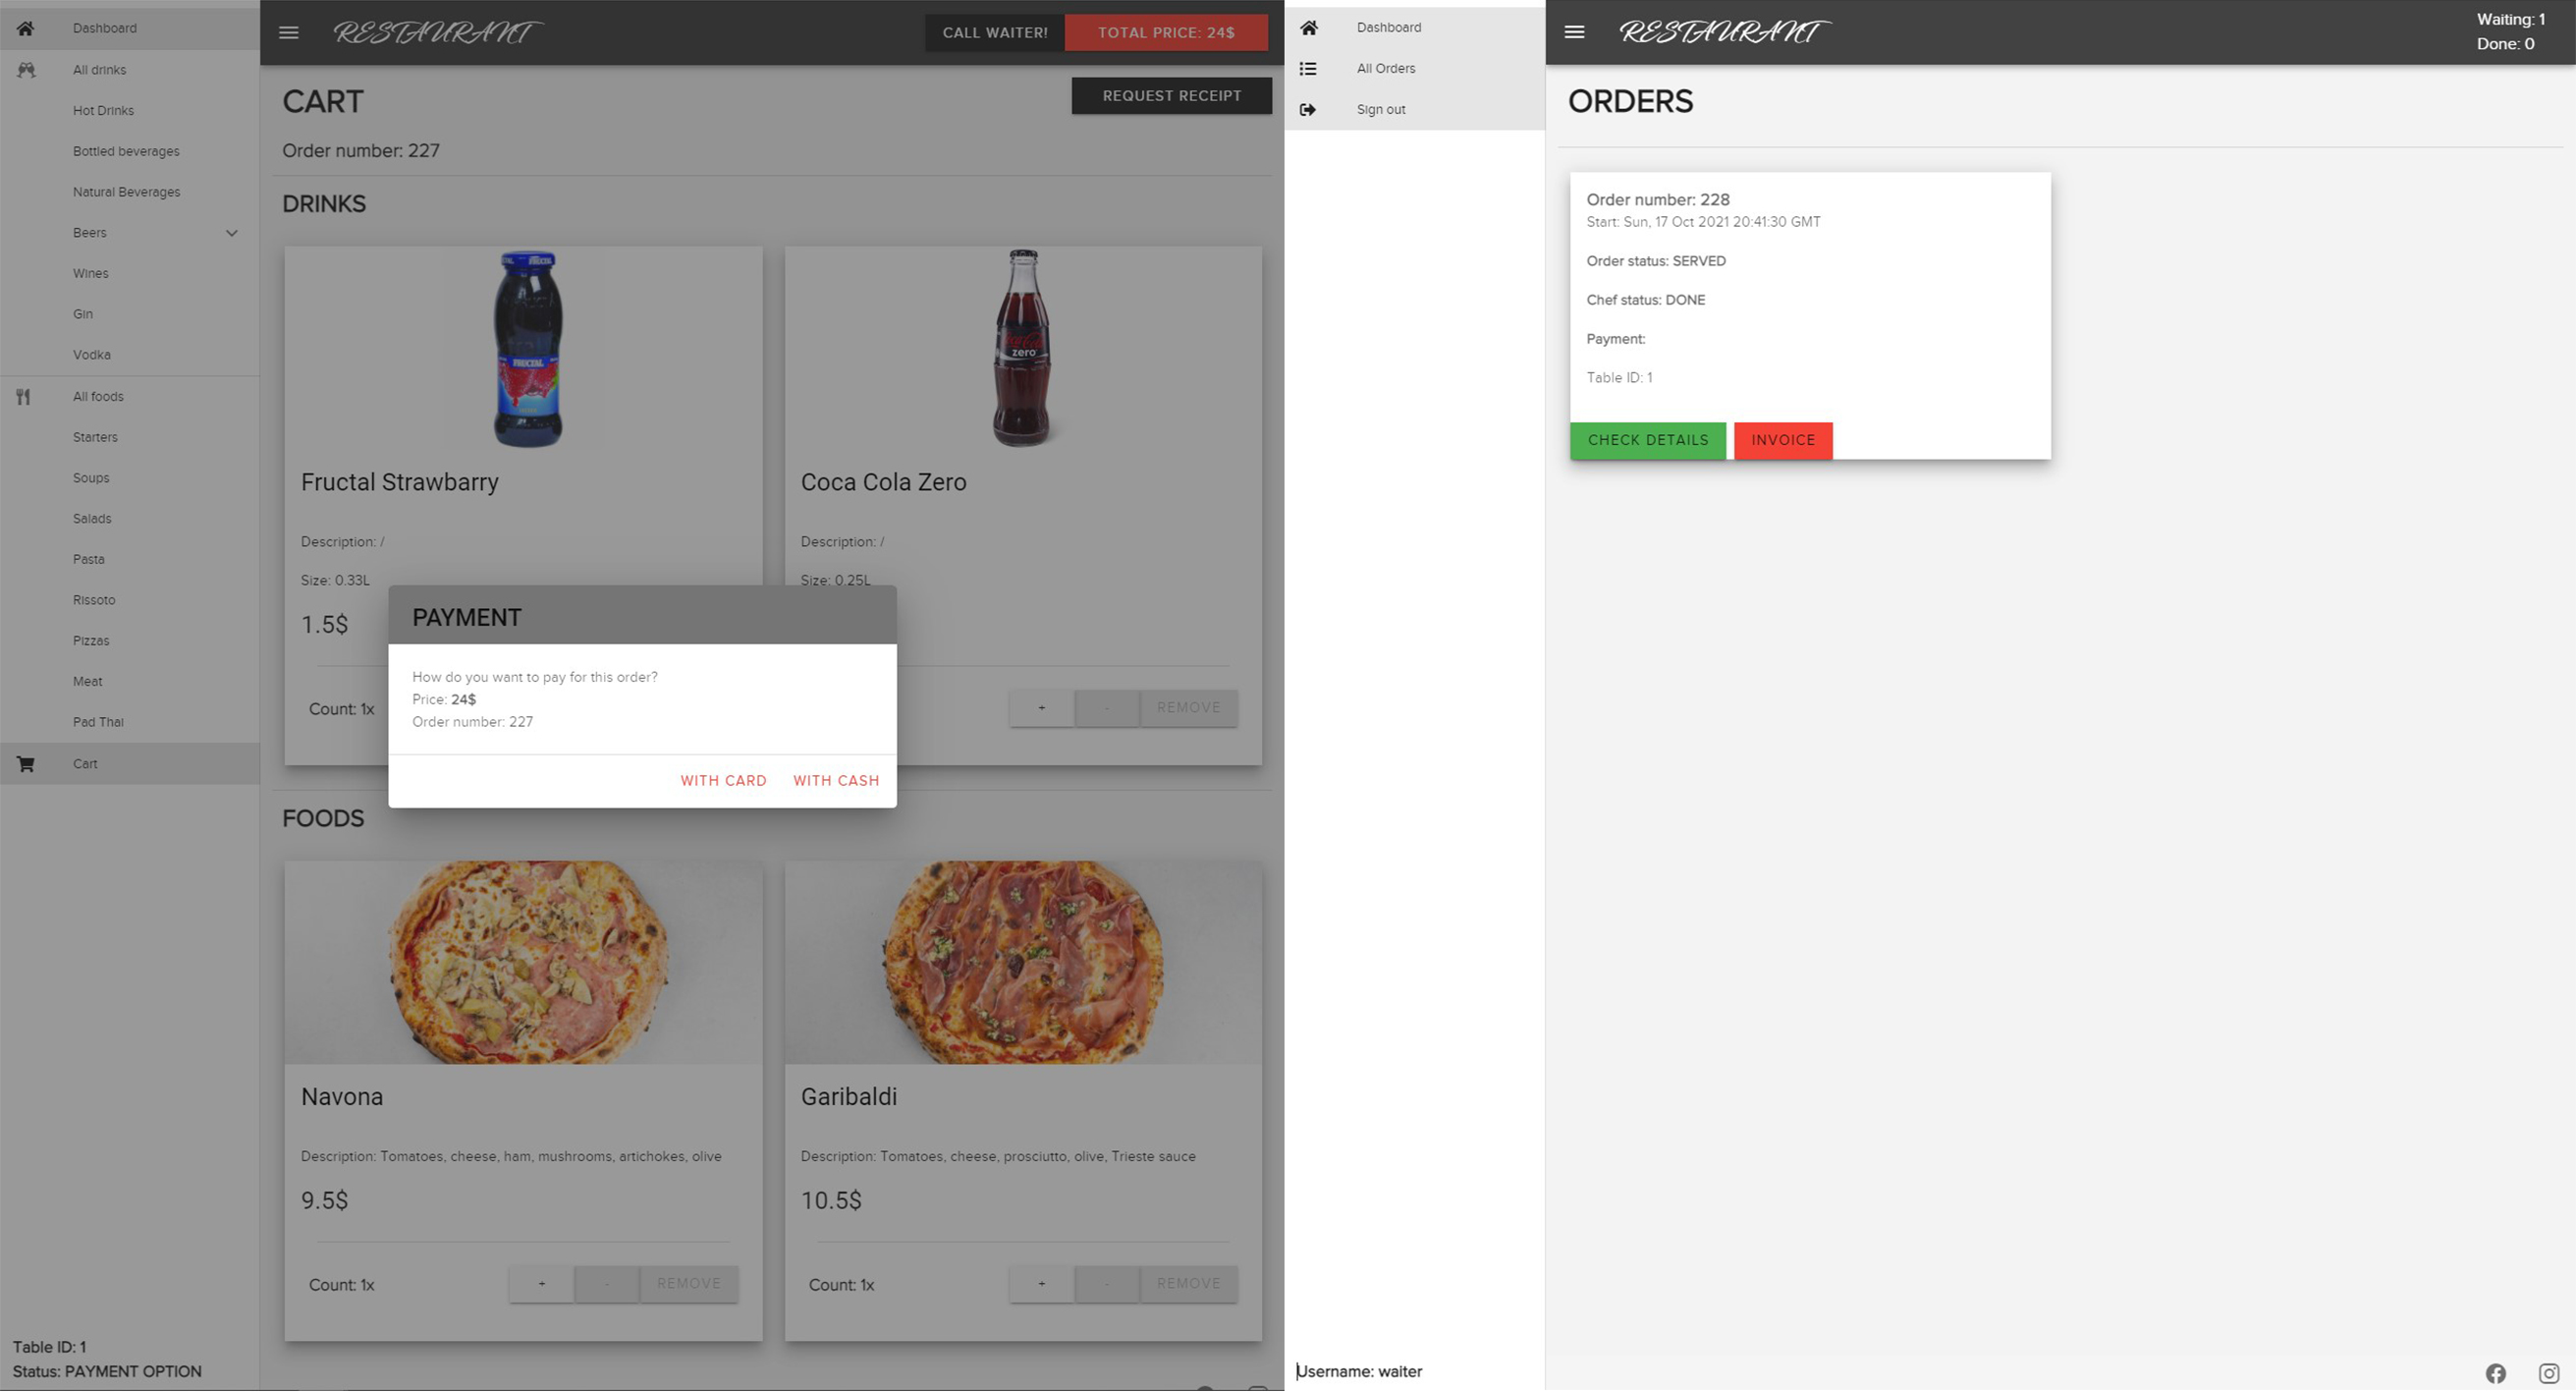
\includegraphics[width=14.5cm]{opis6.jpg}
\caption{Zahtevanje računa}
\label{Opis6}
\end{center}
\end{figure}


\section{Vmesnik za gosta}
Prvi pogled vmesnika za gosta vsebuje napis za dobrodošlico (slika~\ref{Gost}) katerega bi lahko zamenjalo oglaševanja, predstavitev restavracije ali karkoli bi si potencialni kupec zaželel imeti. V zgornjem desnem kotu se nahaja gumb \textit{call waiter} za klic natakarja in števec skupne cene artiklov v nakupovalni košarici. Gumb \textit{call waiter} je namenjena gostom, ki aplikacije ne želijo uporabljati ali v primeru pomoči, če gost pride do kakršnihkoli težav. V spodnjem levem kotu se nahaja status in identifikacijska številka naročila. 
\begin{figure}[!htb]
\begin{center}
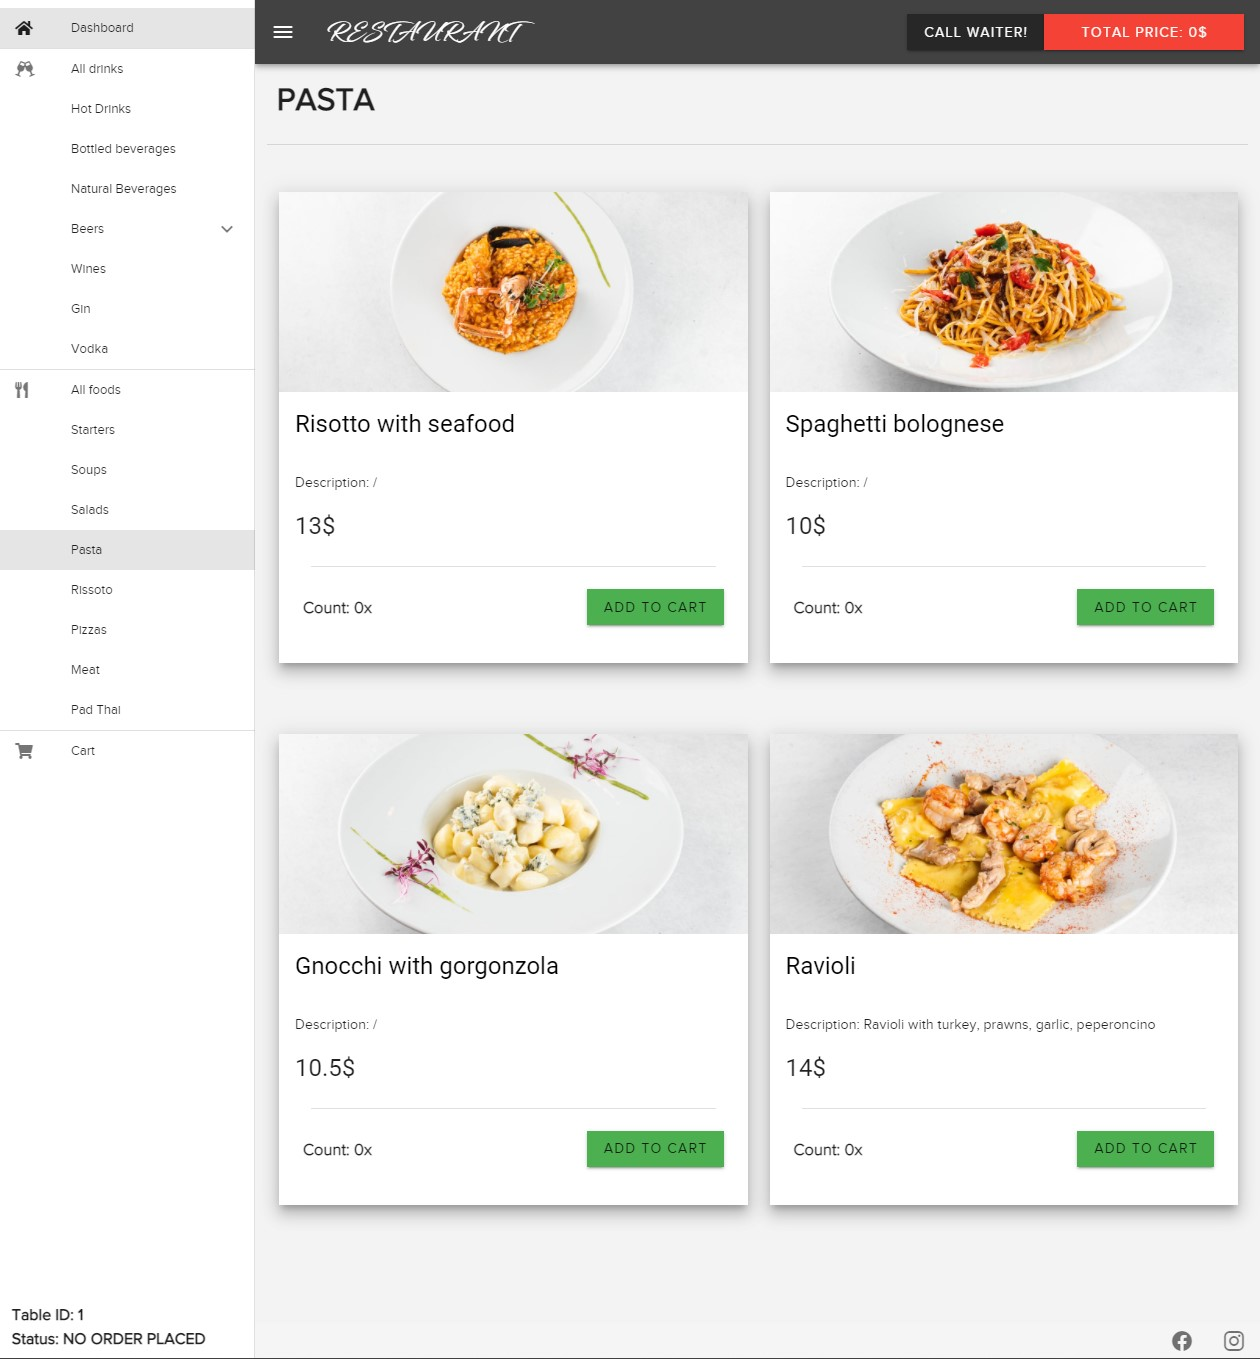
\includegraphics[width=12cm]{gost_3.jpg}
\caption{Seznam artiklov znotraj vrste špagetov}
\label{Gost_3}
\end{center}
\end{figure}

Zavihki na levi strani predstavljajo seznam vseh vrst hrane in pijače, katere kažejo na podstrani ponube, ki jo nudi restavracija (slika~\ref{Gost_3}). Gostu to predstavlja ponudbo s katero v nakupovalno košarico dodaja, briše hrano in pijačo ali spreminja njihovo količino.
\begin{figure}[!htb]
\begin{center}
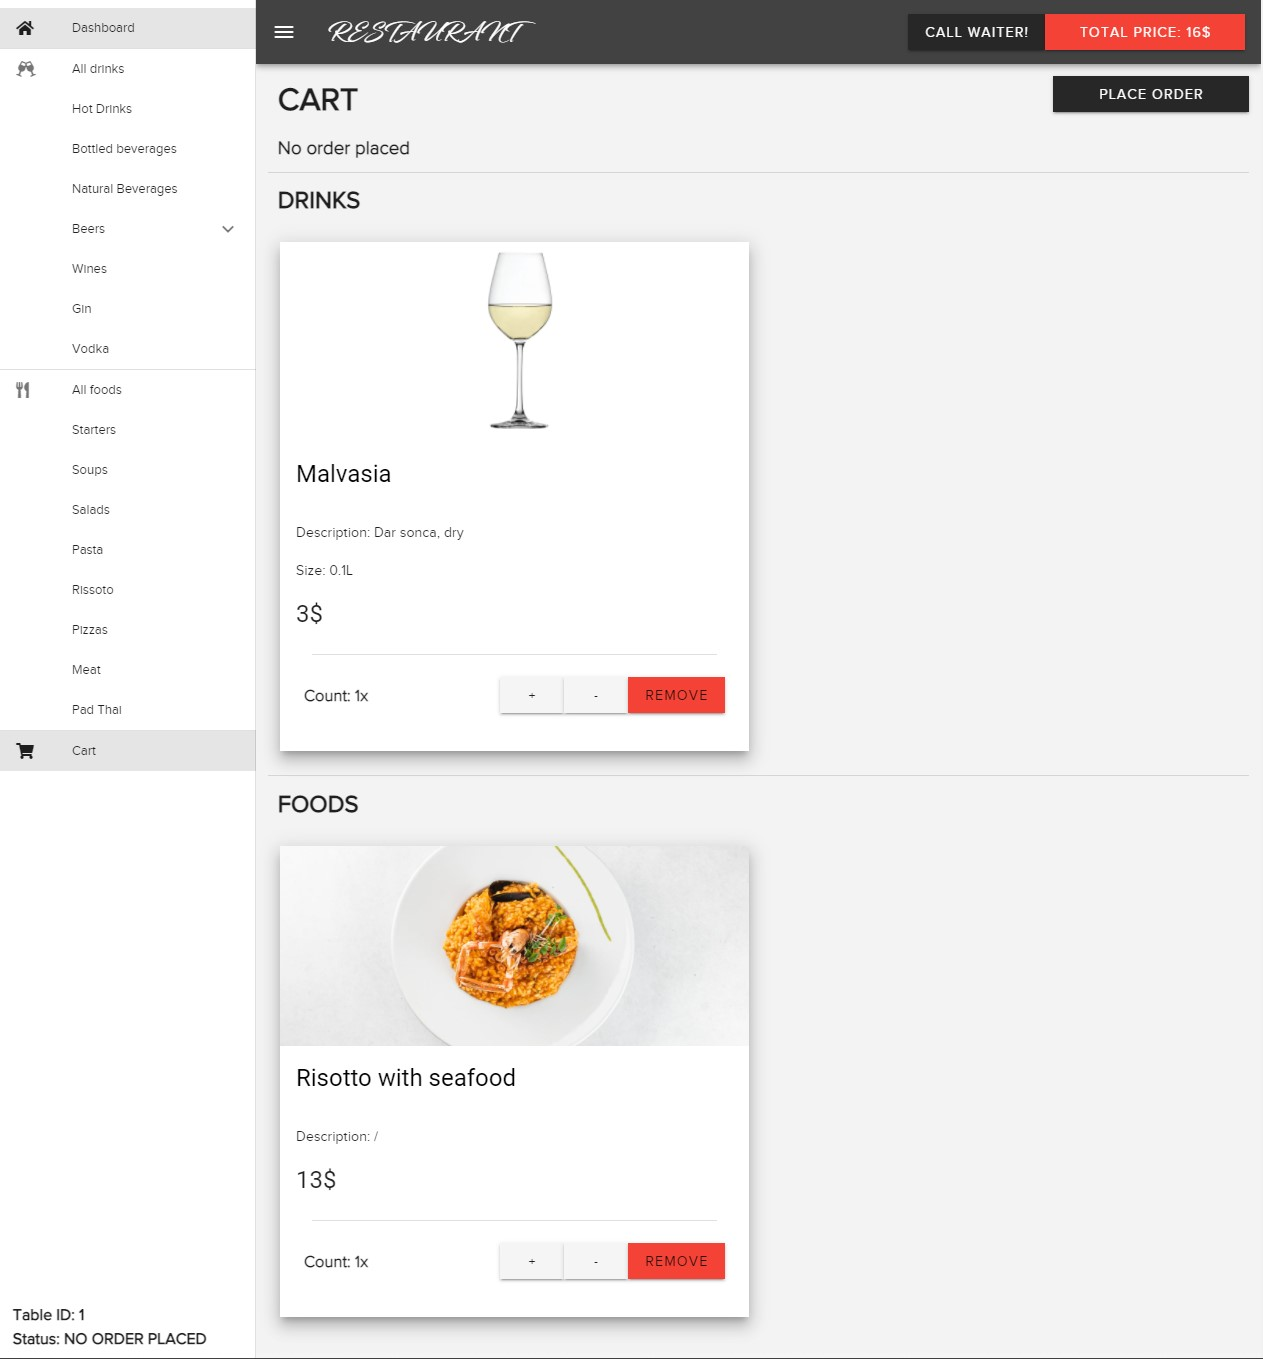
\includegraphics[width=12cm]{gost_4.jpg}
\caption{Primer naročila}
\label{Gost_4}
\end{center}
\end{figure}
 
Vsaka hrana ali pijača vsebuje sliko, ime, opis in ceno. Poleg tega vsebuje še gumb \textit{add to cart} (dodaj v košarico), ki ob kliku izgine in prikaže tri nove gumbe \textit{+} (povečaj količno), \textit{-} (zmanjšaj količino) in \textit{remove} (odstrani). Nakupovalna košarica oziroma \textit{cart} je skupno mesto vse hrane in pijače potencialne za naročilo (slika~\ref{Gost_4}).

Naročilo se odda s klikom na gumb \textit{place order}, ki gosta preusmeri na prvo stran in obvesti s pojavnim sporočilom prikazanim na sliki~\ref{Gost_5}. Ko je naročilo oddano lahko gost ponovno dodaja hrano in pijačo v košarico, vendar je že oddani hrani in pijači onemogočeno zmanjšati količino ali jih izbrisati. Naročilo je sprejeto ko ga natakar potrdi, kar spremeni status naročila in prikaže pojavno sporočilo prikazano na sliki~\ref{Gost_6}. V primeru, da natakar zavrne naročilo, ga mora gost pregledati in ponovno oddati. Tudi v tem primeru je gost obveščen s statusom in pojavnim sporočilom na sliki~\ref{Gost_8}. Naročilo se zaključi s klikom na gumb \textit{request receipt}, ki odpre pojavno okno (slika~\ref{Gost_7}) na katerem je potrebno izbrati način plačila.


\begin{figure}[!htb]
\begin{center}

\includegraphics[width=8.5cm]{gost_5.jpg}
\caption{Pojavno sporočilo ob uspešni oddaji naročila}
\label{Gost_5}
\end{center}
\end{figure}
\begin{figure}[!htb]
\begin{center}

\includegraphics[width=8.5cm]{gost_6.jpg}
\caption{Pojavno sporočilo ob potrditvi naročila s strani natakarja}
\label{Gost_6}
\end{center}
\end{figure}

\begin{figure}[!htb]
\begin{center}
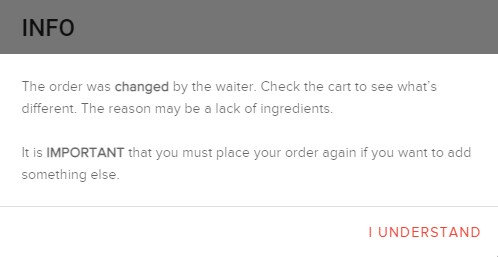
\includegraphics[width=9cm]{gost_8.jpg}
\caption{Pojavno sporočilo ob zavrnitvi naročila s strani natakarja}
\label{Gost_8}
\end{center}
\end{figure}
\begin{figure}[!htb]
\begin{center}

\includegraphics[width=9cm]{gost_7.jpg}
\caption{Pojavno okno z možnostjo izbire načina plačila}
\label{Gost_7}
\end{center}
\end{figure}


\section{Vmesnik za natakarja in kuharja}
Prvi pogled vmesnika je enak tako za natakarja kot kuharja, saj gre za skupno aplikacijo kjer se pogledi razlikujejo glede vlogo uporabnika, ki je določena v podatkovni bazi. Nismo naredili ločene aplikacije, saj ni bilo potrebe, namreč oba uporabnika imata zelo podobne funkcije. Slika~\ref{NatakarGost} prikazuje prijavno okno. Po prijavi natakarja ali kuharja se uporabniško ime izpiše v levem spodnjem kotu. Na zgornji levi strani se prikaže zavihek z dvema podstranema in odjavnim gumbom \textit{sing out}. Prva podstran imenovana \textit{dashboard} ali prva stran ob uspešni prijavi, prikazuje napis za hitrejšo razlikovanje med vlogami. Natakar ima poleg tega v desnem zgornjem kotu še števec čakajočih in zaključenih naročil.

Kuharju se v zavihku \textit{food orders} pojavijo vsa nezaključena naročila, ki vsebujejo hrano (slika ~\ref{Kuhar_4}). Vsako naročilo vsebuje naslednje podatke: identifikacijska številka naročila, čas oddaje naročila, status kuharja in številka mize. Kuhar mora naročilo najprej pregledati z gumbom \textit{check details} (slika  ~\ref{Kuhar_3}) ter ga sprejeti ali zavrniti z gumbom \textit{confirm} in \textit{unconfirm}. Naročilo lahko kuhar zavrne v primeru pomanjkanja sestavin. Ko kuhar zaključi s pripravo hrane o tem obvesti natakarja s klikom na gumb \textit{done}, ki izbriše naročilo iz seznama. Ob vsaki izvedeni akciji se pri vsakem naročilu spremi status kuharja, ki je lahko: \textit{updated}, \textit{confirmed}, \textit{unconfirmed} in \textit{done}. Status \textit{updated} je v primeru dodajanja artiklov k naročilu s strani gosta.

\begin{figure}[!htb]
\begin{center}
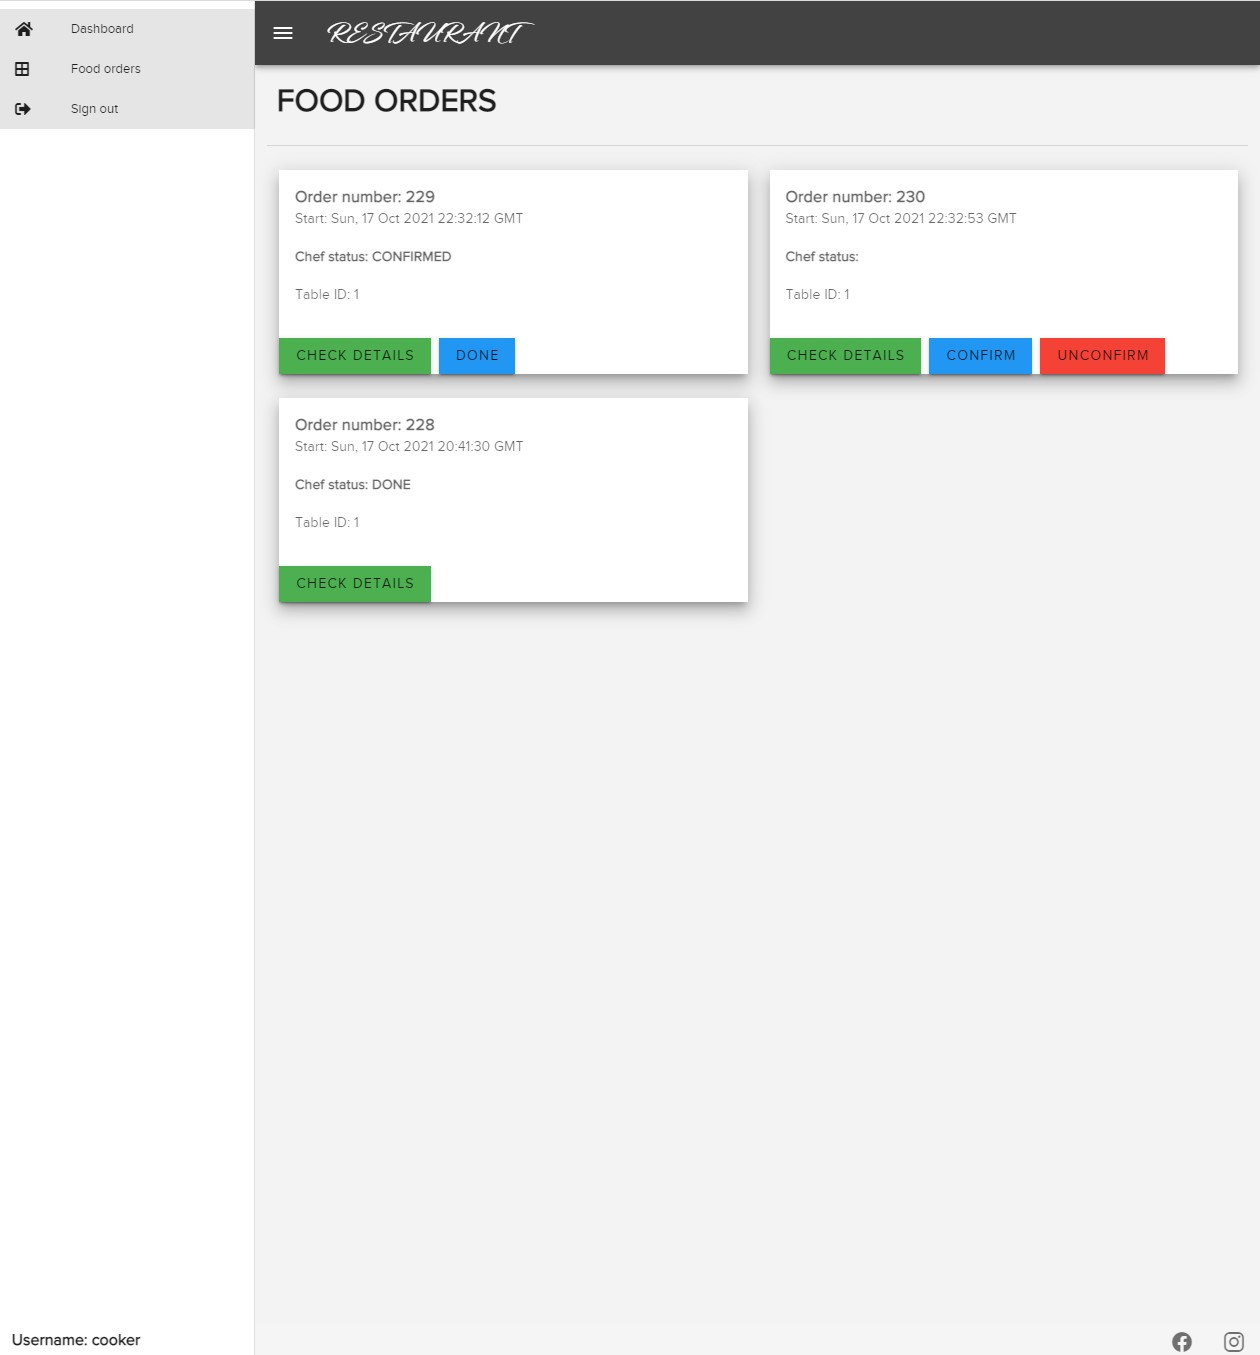
\includegraphics[width=12cm]{kuhar_22.jpg}
\caption{Zavihek \textit{food orders}}
\label{Kuhar_4}
\end{center}
\end{figure}

\begin{figure}[!htb]
\begin{center}
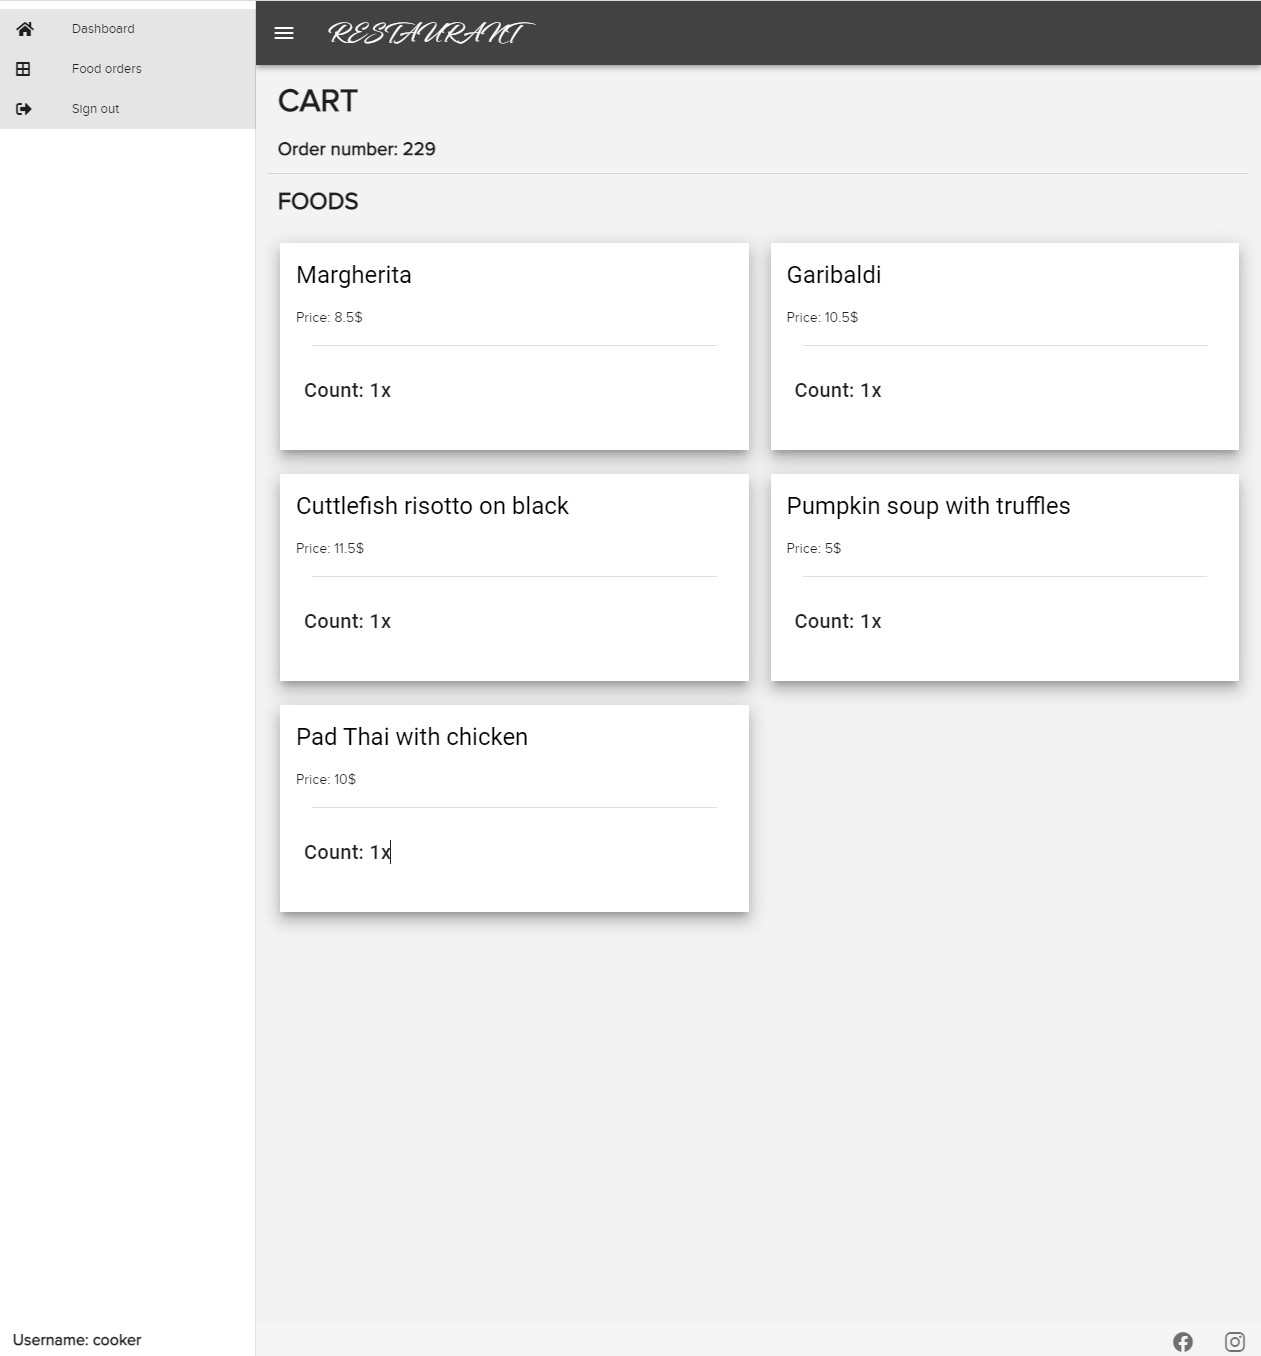
\includegraphics[width=12cm]{kuhar_23.jpg}
\caption{Zavihek, ki se odpre kuharju ob kliku na gumb \textit{check details}}
\label{Kuhar_3}
\end{center}
\end{figure}

Natakarju se v zavihku \textit{all orders} pojavijo vsa nezaključena naročila (slika ~\ref{Natakar_2}). Vsako naročilo vsebuje naslednje podatke: identifikacijska številka naročila, čas oddaje naročila, status naročila, status kuharja, način plačila in številka mize. Izvaja lahko popoln nadzor nad naročili, vendar ob vsaki izvedeni akciji obvesti gosta (slike pojavnih sporočil iz prejšnjega poglavja). Novo naročilo mora natakar najprej potrditi ali zavrniti z gumbom \textit{confirm} ali \textit{unconfirm} oziroma urediti z gumbom \textit{check details} (slika~\ref{Natakar_3}). Natakar lahko ureja celotno naročilo, kar pomeni da lahko spreminja količino hrane in pijače ali jo briše iz naročila. Ko zaključi urjanje mora klikniti na gumb \textit{update order}. Celotno naročilo lahko potrdi šele ko dobi kuharjevo potrditev o hrani. Ko je naročilo potrjeno, natakar čaka na kuharjevo potrditev o pripravi hrane, da jo lahko postreže. Natakar postreženo naročilo označi s klikom na gumb \textit{served}. V primeru, da gost zahteva račun, se natakarju izpiše način plačila v zadevi \textit{payment}. Naročilo se zaključi, ko natakar natisne račun s klikom na gumb \textit{invoice}.

\begin{figure}[!htb]
\begin{center}
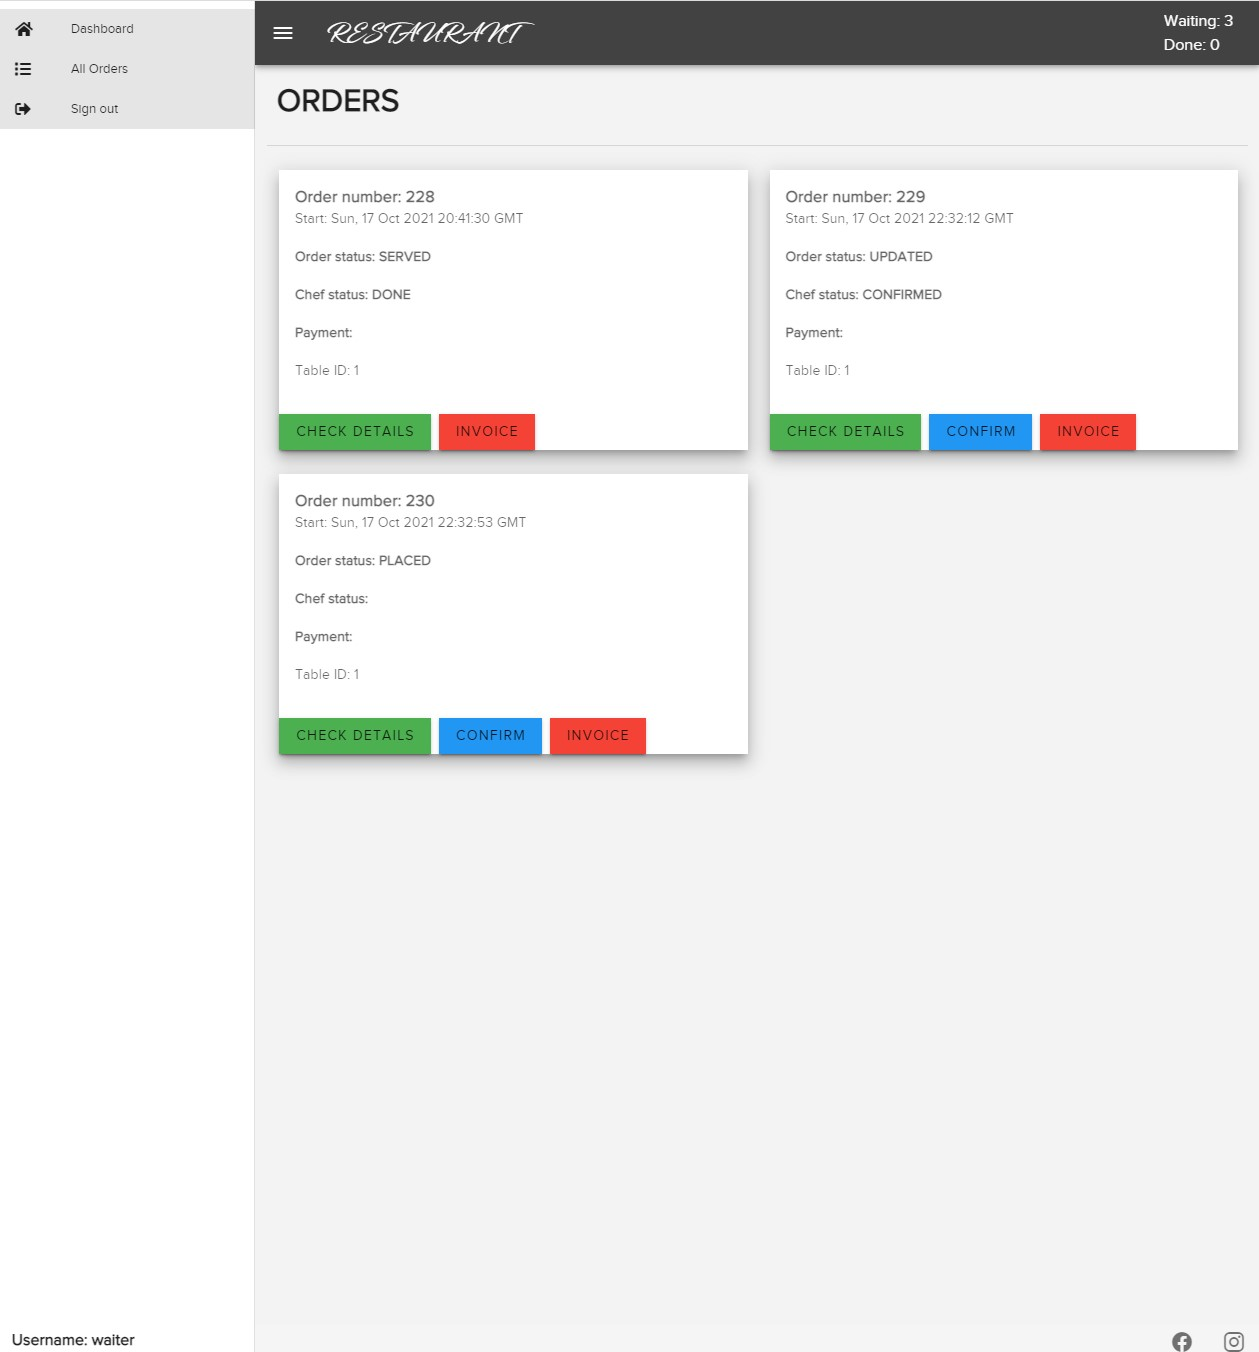
\includegraphics[width=12cm]{natakar_21.jpg}
\caption{Zavihek \textit{all orders}}
\label{Natakar_2}
\end{center}
\end{figure}

\begin{figure}[!htb]
\begin{center}
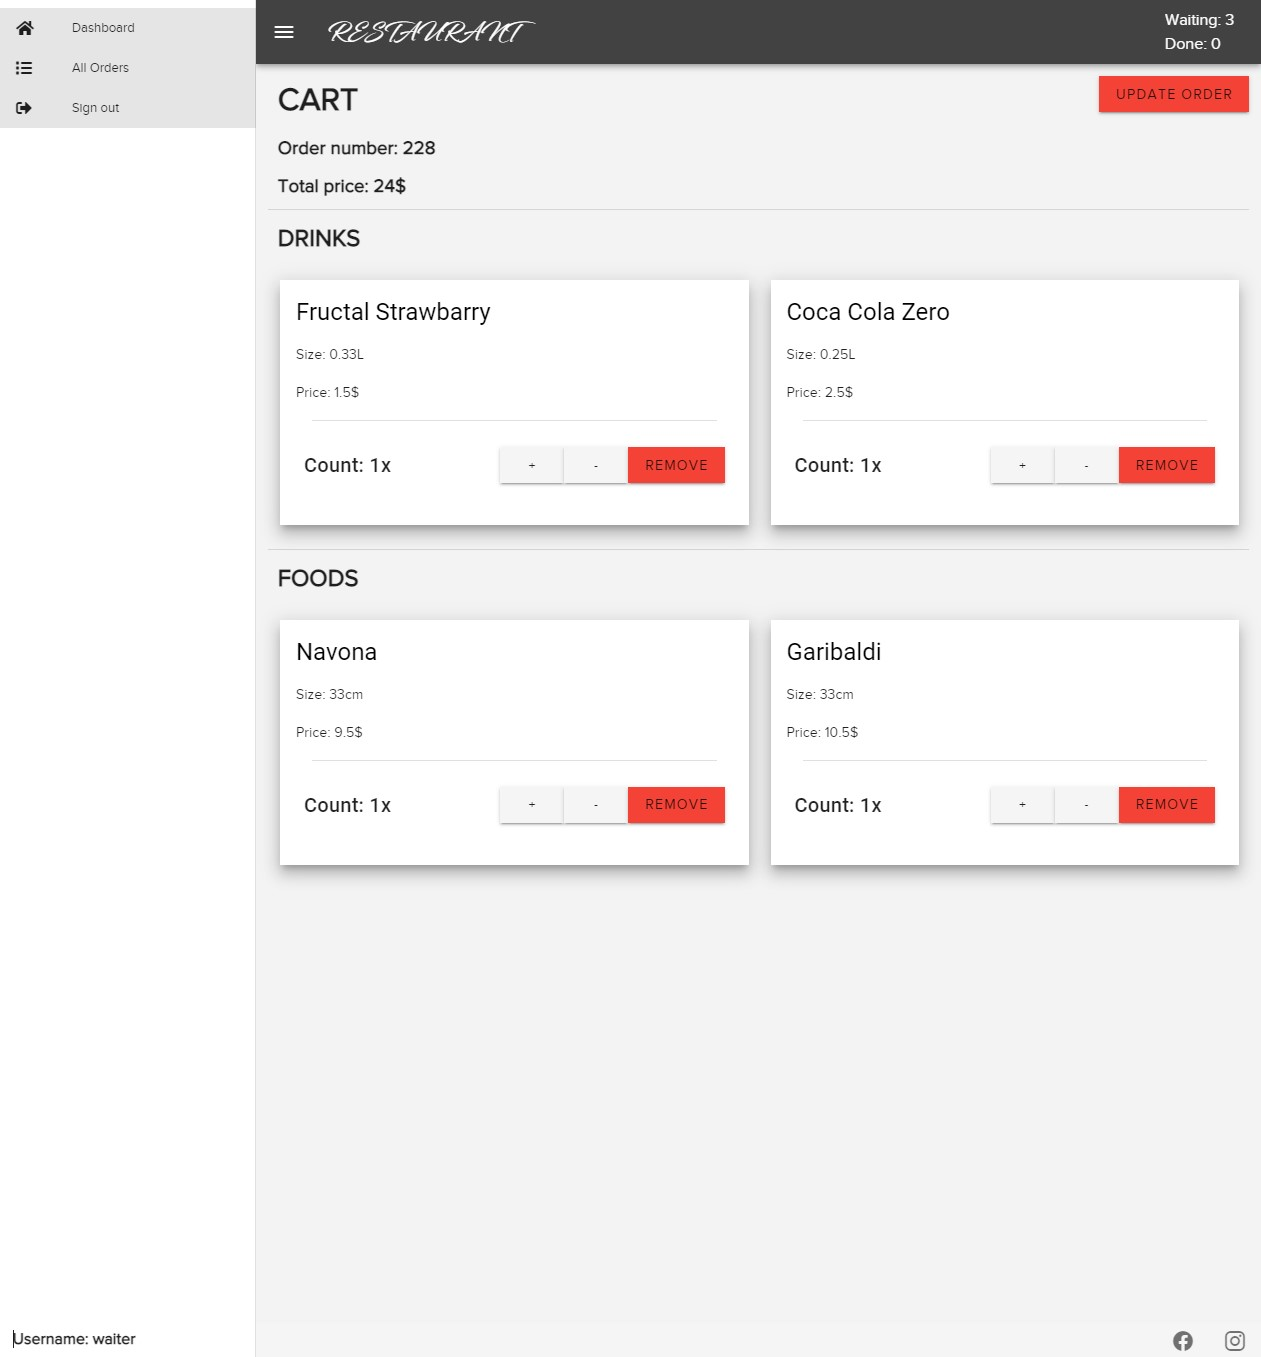
\includegraphics[width=12cm]{natakar_22.jpg}
\caption{Zavihek, ki se odpre natakarju ob kliku na gumb \textit{check details}}
\label{Natakar_3}
\end{center}
\end{figure}




\section{Implementacija programa v realnosti}

Trenutna rešitev omogoča implementacijo znotraj le ene restavracije. Aplikacija bi bila nameščena na lokalnem spletnem strežniku. Naročanje bi gost izvajal s pomočjo tablic, ki bi bile locirane na vsaki mizi v restavraciji. 

Nadgrajena bi predstavljala uporabo aplikacije za naročanje z branjem kode QR (ang. quick response), ki bi bila locirana na vsaki mizi v restavraciji. V kodi bi bilo zapisano ime restavracije in številka mize. Kodo bi gost skeniral z mobitelom in bi bil preusmerjen v aplikacijo. Celoten sistem bi deloval v odprtem internetnem omrežju, tako za goste kot tudi natakarje in kuharje. Strežnik bi bil postavljen za celotno Slovenijo in bi omogočal storitev vsem restavracijam po Sloveniji. Potrebno bi bilo zagotoviti, da ne bi prihajalo do fantomskih naročil, kjer bi nepridipravi oddajali neveljavna naročila. Temu bi se lahko izognili na dva načina. Prvi način bi bil, da bi moral biti uporabnik prijavljen preko lokalnega omrežja s čimer bi overili svojo dejansko prisotnost v restavraciji.
Drugi način bi bilo geslo, ki bi ga uporabnik prejel od natakarja. 


\section{Izboljšave}

Potrebne izboljšave, da bi lahko aplikacijo ponudili potencialnim kupcem so:

1.) Možnost dodajanja hrane in pijače k naročilu s strani vsakega posameznika za mizo.

2.) Možnost hkratnega delovanja več kuharjev, da bi lahko vsak vedel kaj more delati. Tako kot smo to implementirli za natakarje.

3.) Dodatno spremljanje hrane in pijače na strani kuharja/natakarja, kot npr. katera pijača in hrana je že bila postrežena.

4.) Pisanje opomb pri vsakem naročilu, kar bi natakarju in kuharju oljašalo delo ob povečanemu številu gostov.


Napredne izboljšave: 

1.) Statistika za lastnika restavracije, ki bi poleg vseh podatkov računala oceno nabave za prihodnji mesec.

2.) Brezstično plačevanje s plačilno kartico neposredno na strani gosta.

3.) Če bi aplikacija delovala v odprtem internetnem omrežju, bi s pomočjo skupne spletne strani omogočali dostavo hrane za vsako restavracijo.



\chapter {Sklepne ugotovitve}
\newpage %dodaj po potrebi, da bo številka strani za Literaturo v Kazalu pravilna!
\ \\
\clearpage
\addcontentsline{toc}{chapter}{Literatura}
\bibliographystyle{plain}
\bibliography{literatura}


\end{document}

